% \documentclass{article}
% \usepackage{amsmath}
% \usepackage{fancyhdr}
% \usepackage{graphicx}
% \usepackage[utf8]{inputenc}   % Để hỗ trợ Unicode
% \usepackage[T5]{fontenc}       % Để hỗ trợ các ký tự tiếng Việt
% \usepackage[vietnam]{babel}    % Để sử dụng ngôn ngữ tiếng Việt
% FORMAT AND PACKAGES
% {
\documentclass[a4paper]{article}
\usepackage{a4wide,amssymb,epsfig,latexsym,multicol,array,hhline,fancyhdr}
\usepackage{vntex}
\usepackage{amsmath}
\usepackage{lastpage}
\usepackage[lined,boxed,commentsnumbered]{algorithm2e}
\usepackage{enumerate}
\usepackage{listings}
\usepackage{xcolor}
\usepackage{graphicx}							% Standard graphics package
\usepackage{array}
\usepackage{tabularx, caption}
\usepackage{multirow}
\usepackage{multicol}
\usepackage{rotating}
\usepackage{graphics}
\usepackage{geometry}
\usepackage{footnote}
\usepackage{setspace}
\usepackage{epsfig}
\usepackage{tikz}
\usepackage{xfrac}
\usepackage{indentfirst}
\usepackage{tikz}
\usetikzlibrary{shapes, arrows, positioning, fit, calc}
\usetikzlibrary{calc}
\usepackage{bm}
\usepackage{float} % Thêm vào phần preamble
\usepackage[backend=bibtex,style=ieee]{biblatex}
\addbibresource{references.bib} % Include the .bib file
\usepackage[colorlinks]{hyperref}
% \setlength{\parskip}{4pt} % 6pt là một khoảng cách vừa phải, mày có thể tăng/giảm
% \usepackage[acronym,toc]{glossaries}
% \usepackage[symbols,nogroupskip,nonumberlist]{glossaries-extra}
\usepackage[
 sort=none,% no sorting or indexing required
 abbreviations,% create list of abbreviations
 symbols,% create list of symbols
 stylemods,style=list, % set the default glossary style
 nogroupskip, nonumberlist, nomain
]{glossaries-extra}

% Define custom colors for better visibility
\definecolor{codegray}{rgb}{0.5,0.5,0.5}
\definecolor{codepurple}{rgb}{0.6,0.2,0.6}
\definecolor{backcolor}{rgb}{0.95,0.95,0.95}
\def\labelitemi{--}
% Customize the style of the code block
\lstdefinestyle{custom}{
    backgroundcolor=\color{backcolor},  
    commentstyle=\color{codegray},
    keywordstyle=\color{blue},
    stringstyle=\color{codepurple},
    basicstyle=\ttfamily\small,
    breakatwhitespace=false,         
    breaklines=true,                 
    captionpos=b,
    keepspaces=true,
    numbers=left,
    numberstyle=\tiny\color{codegray},
    rulecolor=\color{black},
    showspaces=false,               
    showstringspaces=false,
    showtabs=false,
    tabsize=2
}

\lstset{style=custom}
% FORMATTING
% {
\DeclareMathOperator{\arccot}{arccot}
\captionsetup[table]{name=Table}
\captionsetup[figure]{name=Figure}
\newenvironment{Description}{\list{}{%
    \let\makelabel\descriptionlabel    % this comes from the original description environment
    \setlength{\rightmargin}{\leftmargin}% this comes from the original quote environment
    \setlength{\labelwidth}{0pt}%          this is new
    }}{\endlist}

\hypersetup{urlcolor=blue,linkcolor=black,citecolor=black,colorlinks=true} 
\usetikzlibrary{arrows,snakes,backgrounds}
\definecolor{mathblue}{RGB}{0,114,188}
% \makeatletter  \def\m@th{\mathsurround\z@\color{mathblue}} \makeatother
% \everymath{\color{mathblue}}
% \setmathfont[Color=000000]{Arial}
%\usepackage{pstcol} 								% PSTricks with the standard color package
\newtheorem{theorem}{{\bf Theorem}}
\newtheorem{property}{{\bf Property}}
\newtheorem{proposition}{{\bf Proposition}}
\newtheorem{corollary}[proposition]{{\bf Corollary}}
\newtheorem{lemma}[proposition]{{\bf Lemma}}
%\usepackage{fancyhdr}
% Định nghĩa header và footer
\setlength{\headheight}{40pt}
\pagestyle{fancy}
\fancyhead{} % clear all header fields
\fancyhead[L]{
 \begin{tabular}{rl}
    \begin{picture}(25,15)(0,0)
    \put(0,-8){\includegraphics[width=10mm, height=10mm]{hcmut.jpg}}
    %\put(0,-8){\epsfig{width=10mm,figure=hcmut.eps}}
   \end{picture}&
	%\includegraphics[width=8mm, height=8mm]{hcmut.png} & %
	\begin{tabular}{l}
		\textbf{\bf \ttfamily University of Technology, Ho Chi Minh City}\\
		\textbf{\bf \ttfamily Faculty of Computer Science and Engineering}
	\end{tabular} 	
 \end{tabular}
}
\fancyhead[R]{
	\begin{tabular}{l}
		\tiny \bf \\
		\tiny \bf 
	\end{tabular}  }
\fancyfoot{} % clear all footer fields
\fancyfoot[L]{\scriptsize \ttfamily Báo cáo đồ án tổng hợp - HK251}
\fancyfoot[R]{\scriptsize \ttfamily Page {\thepage}/\pageref{LastPage}}
\renewcommand{\headrulewidth}{0.3pt}
\renewcommand{\footrulewidth}{0.3pt}


\setcounter{secnumdepth}{4}
\setcounter{tocdepth}{4}

\begin{document}
\begin{titlepage}
\begin{tikzpicture}[remember picture,overlay]
  \draw[line width=2pt] 
    ($(current page.north west) + (1cm,-1cm)$) rectangle 
    ($(current page.south east) + (-1cm,1cm)$);
\end{tikzpicture}
\begin{center}
{\Large \textbf{ĐẠI HỌC QUỐC GIA THÀNH PHỐ HỒ CHÍ MINH}}\\[0.3cm]
    {\Large \textbf{TRƯỜNG ĐẠI HỌC BÁCH KHOA}}\\[0.3cm]
    {\large \textbf{KHOA KHOA HỌC - KỸ THUẬT MÁY TÍNH}}\\[1cm]
\end{center}

\vspace{0.5cm}

\begin{figure}[h!]
\begin{center}
\includegraphics[width=4cm]{hcmut.jpg}
\end{center}
\end{figure}
\vspace{0.5cm}
\begin{flushleft}
    \large \textbf{BÁO CÁO ĐỒ ÁN TỔNG HỢP - HƯỚNG TRÍ TUỆ NHÂN TẠO} \\
    \rule{\linewidth}{0.3pt} \\
    \begin{center}
        \huge \textbf{Reinforcement Learning: lịch sử, cơ sở lý thuyết cho đến ứng dụng và nghiên cứu, định hướng trong tương lai} \\
        \rule{\linewidth}{0.3pt}
    \end{center}
\end{flushleft}

\vspace{1cm}

\begin{table}[h]
\centering
\renewcommand{\arraystretch}{1.7} % giãn dòng cho dễ nhìn
\setlength{\tabcolsep}{10pt} % khoảng cách cột
\begin{tabular}{|p{7cm}|p{7cm}|}
% \hline
% \multicolumn{2}{|c|}{\textbf{THÔNG TIN HƯỚNG DẪN VÀ SINH VIÊN}}\\
\hline
\textbf{Giảng viên hướng dẫn} & TS. Nguyễn Đức Dũng \\ 
\hline
\textbf{Sinh viên thực hiện} & Phạm Quang Hiếu -- 2310974 \\
\hline
\end{tabular}
\end{table}


\vspace{1cm}
\begin{center}
{\footnotesize TP. HỒ CHÍ MINH, THÁNG 11/2025}
\end{center}
\end{titlepage}

\tableofcontents
\newpage

\section{Giới thiệu}

Reinforcement Learning (RL) là một nhánh quan trọng của học máy, tập trung vào việc huấn luyện các tác nhân (agent) học cách ra quyết định thông qua tương tác với môi trường nhằm tối đa hóa tổng phần thưởng tích lũy theo thời gian . Khác với học có giám sát (supervised learning) yêu cầu dữ liệu gắn nhãn sẵn hoặc học không giám sát (unsupervised learning) tìm kiếm cấu trúc ẩn trong dữ liệu, RL dựa trên nguyên tắc \textit{thử và sai} (trial-and-error) kết hợp với cơ chế thưởng phạt, gần giống với cách con người và động vật học từ kinh nghiệm thực tế.\cite{sutton2018reinforcement}
\cite{datarootlabs_rl_state}
\begin{figure}[H]
    \centering
    \includegraphics[width=0.7\linewidth]{1.png}
    \caption{Vòng lặp tương tác cơ bản giữa Tác nhân và Môi trường trong RL.}
\end{figure}


\subsection{Những thành tựu nổi bật về Reinforcement Learning}

Trong thập kỷ qua, RL đã đạt được những bước tiến vượt bậc nhờ sự kết hợp với mạng nơ-ron sâu (Deep Reinforcement Learning). Các cột mốc nổi bật bao gồm AlphaGo của DeepMind đánh bại kỳ thủ hàng đầu thế giới Lee Sedol năm 2016, AlphaStar thống trị StarCraft II, và gần đây nhất là việc áp dụng RL từ phản hồi con người (RLHF) để tinh chỉnh các mô hình ngôn ngữ lớn (LLM) như ChatGPT hay Grok, giúp chúng tạo ra phản hồi an toàn, hữu ích và phù hợp hơn với sở thích người dùng. Đến năm 2025, các mô hình như OpenAI o1 đã sử dụng RL để tăng cường khả năng suy luận chuỗi tư duy (chain-of-thought reasoning), đạt hiệu suất vượt trội trên các benchmark toán học và lập trình phức tạp.

Sự bùng nổ của RL không chỉ giới hạn trong trò chơi điện tử mà đã mở rộng sang nhiều lĩnh vực thực tiễn: robot (học điều khiển chuyển động), y tế (tối ưu phác đồ điều trị), tài chính (giao dịch thuật toán), giao thông (điều khiển đèn tín hiệu thông minh), và gần đây nhất là tích hợp với Generative AI để tạo ra nội dung sáng tạo có mục tiêu cụ thể. Những thành tựu này đã biến RL từ một lĩnh vực lý thuyết thành công cụ cốt lõi trong hành trình hướng tới Trí tuệ Nhân tạo Tổng quát (AGI).
\cite{datarootlabs_rl_state}

\subsection{Sơ bộ về bài báo cáo}
\textbf{Mục tiêu của báo cáo} là cung cấp cái nhìn toàn diện về Reinforcement Learning, từ nền tảng lịch sử và lý thuyết đến các ứng dụng thực tiễn, phân tích nghiên cứu mới nhất, và định hướng phát triển trong tương lai. Thông qua dự án thực hành và review các công trình tiêu biểu, báo cáo nhằm làm rõ tiềm năng cũng như thách thức còn tồn tại của RL trong bối cảnh công nghệ AI năm 2025.\newline

\textbf{Cấu trúc báo cáo} được tổ chức thành bảy phần chính:
\begin{enumerate}
    \item Giới thiệu (phần hiện tại).
    \item Lịch sử và ý tưởng cơ bản của Reinforcement Learning.
    \item Ví dụ về Reinforcement Learning và dự án thực hành.
    \item Review các công trình nghiên cứu gần đây về RL trong Generative AI, tập trung vào RLHF và mô hình reasoning, World Models.
    \item Reinforcement Learning: Ứng dụng trong thực tiễn
    \item Định hướng phát triển và thách thức trong tương lai.
    \item Kết luận và tài liệu tham khảo.
\end{enumerate}

Qua đó, báo cáo không chỉ tổng hợp kiến thức mà còn trình bày kết quả thực nghiệm cụ thể, góp phần minh họa sức mạnh của RL trong việc giải quyết các bài toán quyết định tuần tự phức tạp.


\section{Lịch sử và Cội nguồn Tư tưởng của Học Tăng Cường}
\label{sec:history_narrative}

Lịch sử của Học tăng cường (Reinforcement Learning - RL) không đơn thuần là sự phát triển tuyến tính của một thuật toán, mà là một bản giao hưởng được hợp thành từ ba dòng chảy tư tưởng lớn của khoa học thế kỷ 20. Ba dòng chảy này, khởi nguồn từ những lĩnh vực hoàn toàn tách biệt—tâm lý học hành vi, lý thuyết điều khiển tối ưu và khoa học máy tính—đã trôi song song trong nhiều thập kỷ trước khi hội tụ để tạo nên nền tảng cho trí tuệ nhân tạo hiện đại.\cite{sutton2018reinforcement}

\subsection{Dòng chảy thứ nhất: Học qua Thử và Sai – Bản năng của sinh tồn}

Dòng chảy đầu tiên và nguyên thủy nhất bắt nguồn từ việc quan sát cách sinh vật học hỏi để sinh tồn. Ngay từ những năm 1850, ý niệm về việc học thông qua "mò mẫm và thử nghiệm" đã nhen nhóm trong tâm lý học. Tuy nhiên, phải đến năm 1911, Edward Thorndike mới chính thức hóa điều này qua "Luật Hiệu ứng" (Law of Effect). Ông quan sát thấy rằng, những hành động mang lại sự thỏa mãn sẽ được khắc sâu vào ký ức, trong khi những hành động gây khó chịu sẽ dần bị đào thải.

Tuy nhiên, thuật ngữ \textit{"Reinforcement"} (Củng cố) mà chúng ta dùng ngày nay lại xuất hiện muộn hơn, lần đầu tiên được tìm thấy trong bản dịch tiếng Anh năm 1927 của Ivan Pavlov về phản xạ có điều kiện. 

Pavlov mô tả sự củng cố là việc làm mạnh thêm một mẫu hành vi khi động vật nhận được một kích thích (reinforcer) theo một trình tự thời gian thích hợp. Một kích thích chỉ được coi là "củng cố" nếu sự thay đổi hành vi mà nó tạo ra tồn tại bền vững ngay cả khi kích thích đó đã rút đi, phân biệt rõ ràng với việc chỉ đơn thuần thu hút sự chú ý nhất thời.

\begin{figure}[H]
    \centering
    % Nhớ đổi tên file ảnh cho đúng với file mày up lên
    \includegraphics[width=0.8\linewidth]{2.png} 
    \caption{\textbf{Hộp Skinner (Skinner Box):} Thí nghiệm sinh học kinh điển minh họa cơ chế cốt lõi của Học tăng cường.\cite{britannica_law_effect}}
    \label{fig:skinner_box}
\end{figure}


\textbf{Phân tích mối liên hệ với Reinforcement Learning:}Hình \ref{fig:skinner_box} mô tả thí nghiệm về \textit{Điều kiện hóa từ hoạt} (Operant Conditioning), đây chính là mô hình vật lý nguyên bản của một bài toán MDP. Sự tương quan cụ thể như sau:
\begin{itemize}
    \item \textbf{Agent (Tác nhân):} Con chuột – đối tượng thực hiện quá trình học.
    \item \textbf{Environment (Môi trường):} Chiếc hộp với các quy luật vật lý ẩn (cơ chế nhả thức ăn hoặc giật điện).
    \item \textbf{State (Trạng thái $s_t$):} Các tín hiệu từ cảm biến như đèn (signal lights) hoặc loa (speaker).
    \item \textbf{Action (Hành động $a_t$):} Quyết định gạt cần (press lever) hoặc không gạt.
    \item \textbf{Reward (Phần thưởng $r_t$):} Viên thức ăn (Reward dương $+1$) để khuyến khích hành vi, hoặc xung điện (Reward âm $-1$) để trừng phạt.
\end{itemize}

Qua quá trình \textit{thử và sai}, con chuột sẽ điều chỉnh hành vi để tìm ra \textbf{Chính sách tối ưu ($\pi^*$)}: gạt cần đúng lúc đèn sáng để nhận thức ăn và tránh bị điện giật.

Tư tưởng này đã thâm nhập vào khoa học máy tính từ rất sớm. Năm 1948, Alan Turing—cha đẻ của Khoa học máy tính—đã phác thảo thiết kế cho một "hệ thống sướng-khổ" (pleasure-pain system). Ông mô tả một cỗ máy biết tự sửa đổi cấu trúc của mình: tín hiệu "đau" sẽ xóa bỏ các lệnh sai lầm, trong khi tín hiệu "sướng" sẽ đóng băng và ghi nhớ các lệnh đúng đắn:
\begin{quote}
    "When a configuration is reached for which the action is undetermined, a random choice for the missing data is made and the appropriate entry is made in the description, tentatively, and is applied. When a pain stimulus occurs all tentative entries are cancelled, and when a pleasure stimulus occurs they are all made permanent." (Turing, 1948)
\end{quote}
Đây chính là tiền thân sơ khai nhất của việc cập nhật trọng số dựa trên phần thưởng trong các thuật toán RL hiện đại.

\subsection{Dòng chảy thứ hai: Bài toán Optimal Control – Sự chính xác của toán học}

Trong khi các nhà tâm lý học quan sát hành vi bên ngoài, thì ở một chiến tuyến khác, các nhà toán học và kỹ sư đang vật lộn với cấu trúc bên trong của việc ra quyết định. Thuật ngữ "Điều khiển tối ưu" (Optimal Control) xuất hiện vào cuối những năm 1950, mô tả bài toán thiết kế một bộ điều khiển nhằm cực tiểu hóa hoặc cực đại hóa một thước đo hành vi của hệ thống động lực theo thời gian.

Richard Bellman là người đã đặt nền móng cho dòng chảy này vào giữa thập niên 1950 bằng cách mở rộng lý thuyết thế kỷ 19 của Hamilton và Jacobi. Ông giới thiệu phương pháp "Lập trình động" (Dynamic Programming) và hai khái niệm cốt lõi: \textit{Trạng thái (State)} của hệ thống và \textit{Hàm giá trị (Value Function)}. Từ đây, phương trình Bellman ra đời—một phương trình đệ quy đẹp đẽ định nghĩa mối quan hệ giữa giá trị hiện tại và tương lai.



Năm 1957, Bellman tiếp tục giới thiệu phiên bản ngẫu nhiên rời rạc của bài toán điều khiển, gọi là \textit{Quy trình Quyết định Markov} (Markov Decision Processes - MDPs). Tiếp nối ông, Ronald Howard (1960) đã phát triển phương pháp \textit{Lặp chính sách} (Policy Iteration) cho MDPs. Tất cả những công cụ này chính là khung xương sống toán học của RL hiện đại.

Tuy nhiên, tại sao dòng chảy này lại tách biệt với "Học tập" (Learning) trong suốt nhiều thập kỷ?
\begin{itemize}
    \item \textbf{Giả định về mô hình hoàn hảo:} Lập trình động truyền thống là một phương pháp tính toán "offline". Nó yêu cầu chúng ta phải biết chính xác mọi quy luật vật lý của môi trường (biết trước mô hình) để giải phương trình Bellman. Nó giống như việc lập kế hoạch chi tiết trên giấy trước khi hành động, chứ không phải vừa làm vừa học.
    \item \textbf{Lời nguyền của số chiều (Curse of Dimensionality):} Bellman đã cay đắng thừa nhận rằng chi phí tính toán của Lập trình động sẽ bùng nổ theo hàm mũ khi số lượng biến trạng thái tăng lên. Điều này khiến nó trở nên bất khả thi với các bài toán phức tạp trong thực tế vào thời điểm đó.
\end{itemize}

Chính vì vậy, Lập trình động đã tồn tại như một lý thuyết toán học uyên bác nhưng xa rời thực tế "thử và sai", cho đến khi Chris Watkins (1989) tìm ra cách kết hợp nó với việc học tập sự, giúp giải phóng nó khỏi yêu cầu về mô hình môi trường hoàn hảo.

\subsection{Dòng chảy thứ ba: Temporal-Difference Learning – Chiếc cầu nối bị lãng quên}

Mảnh ghép cuối cùng và cũng không kém phần quan trọng của bức tranh lịch sử là phương pháp Temporal-Difference Learning. Khác với hai dòng chảy trên, TD không học từ kết quả cuối cùng, mà học từ sự thay đổi trong các dự đoán kế tiếp nhau.

Ý tưởng này được nhen nhóm từ khái niệm "củng cố thứ cấp" (secondary reinforcers) trong thí nghiệm của Pavlov, tức là tiếng chuông báo hiệu cho thức ăn cũng đem lại cảm giác như chính thức ăn nếu đã quen với trải nghiệm đó trong một thời gian dài. Trong lĩnh vực máy tính, Arthur Samuel vào năm 1959 là người đầu tiên hiện thực hóa ý tưởng này qua chương trình chơi cờ Đam (Checkers) nổi tiếng. Chương trình của Samuel có khả năng tự đánh giá lại thế cờ dựa trên các dự đoán của chính nó ở những nước đi sau đó, thay vì đợi đến khi ván cờ kết thúc.

\textbf{Bản chất của TD Learning: "Học từ sự khác biệt giữa dự đoán"}

Để hiểu rõ sự khác biệt giữa ba phương pháp, hãy so sánh cách chúng cập nhật kiến thức:

\begin{figure}[H]
    \centering
    \includegraphics[width=1\linewidth]{5.png}
    \caption{So sánh ba phương pháp học: Dynamic Programming (phải biết toàn bộ mô hình), Monte Carlo (học từ kết quả cuối), và Temporal-Difference (học từng bước ngay lập tức). \cite{TD}}
    \label{fig:td_comparison}
\end{figure}

\begin{itemize}
    \item \textbf{Dynamic Programming (Lập trình động):} Yêu cầu biết trước toàn bộ mô hình môi trường (xác suất chuyển trạng thái và phần thưởng). Giống như việc có một bản đồ hoàn chỉnh trước khi lên kế hoạch. Cập nhật giá trị dựa trên \textit{kỳ vọng toán học} của tất cả trạng thái kế tiếp có thể xảy ra:
    \begin{equation}
        V(s_t) \leftarrow E_\pi[r_{t+1} + \gamma V(s_{t+1})]
    \end{equation}
    
    \item \textbf{Monte Carlo Learning:} Không cần biết mô hình, nhưng phải đợi đến \textit{cuối tập} (episode) để cập nhật. Giống như việc đi hết cả chặng đường rồi mới rút kinh nghiệm. Cập nhật giá trị dựa trên \textit{tổng phần thưởng thực tế} $R_t$ nhận được:
    \begin{equation}
        V(s_t) \leftarrow V(s_t) + \alpha[R_t - V(s_t)]
    \end{equation}
    
    \item \textbf{Temporal-Difference Learning:} Kết hợp ưu điểm của cả hai. Không cần mô hình như Monte Carlo, nhưng cập nhật \textit{ngay lập tức} sau mỗi bước như Dynamic Programming. Học từ \textit{sự khác biệt} giữa dự đoán hiện tại và dự đoán ở bước kế tiếp:
    \begin{equation}
        V(s_t) \leftarrow V(s_t) + \alpha[r_{t+1} + \gamma V(s_{t+1}) - V(s_t)]
    \end{equation}
\end{itemize}

Công thức TD có thể được hiểu như một câu hỏi: \textit{"Phần thưởng vừa nhận + Giá trị dự đoán của trạng thái mới có khớp với dự đoán cũ của tôi không?"} Nếu không khớp, điều chỉnh ngay. Đây chính là lý do TD được gọi là phương pháp "bootstrapping" – nó tự kéo mình lên bằng cách học từ chính ước lượng của bản thân.

\textbf{Ý nghĩa lịch sử:} 
Chương trình chơi cờ Đam của Samuel là minh chứng sống động nhất cho sức mạnh của TD. Thay vì chơi hàng triệu ván để biết thế nào là "thắng" (Monte Carlo), chương trình của ông tự đánh giá: "Nếu nước đi này khiến thế cờ sau tốt hơn thế cờ trước, thì nước đi này đáng giá!". Đây là tinh thần của Temporal-Difference – học từ quá trình, không chờ đợi kết quả.

\subsection{Sự hội tụ và Kỷ nguyên mới của Reinforcement learning}

Cuối những năm 1980 đánh dấu thời điểm lịch sử khi ba dòng chảy này hòa làm một. Harry Klopf đã nỗ lực khôi phục lại tầm quan trọng của việc học "thử và sai" trong AI. Cùng lúc đó, Sutton và Barto đã phát triển các thuật toán TD, kết nối toán học của Bellman với trực giác tâm lý học.

Năm 1989, Chris Watkins tạo ra bước đột phá với thuật toán Q-learning. Lần đầu tiên, nhân loại có một phương pháp cho phép máy tính học được chính sách tối ưu (từ dòng chảy Điều khiển tối ưu) thông qua thử và sai (từ dòng chảy Tâm lý học) mà không cần biết trước mô hình môi trường, sử dụng cơ chế cập nhật của TD learning. Sự hội tụ này đã mở toang cánh cửa cho kỷ nguyên hiện đại.

Những thành tựu vang dội sau này, từ TD-Gammon (1992) đánh bại các kiện tướng Backgammon, cho đến cú nổ lớn Deep Q-Network (DQN) của DeepMind năm 2015 và chiến thắng của AlphaGo năm 2016, đều là những bước tiến cho quan trọng sự bùng nổ và phát triển của Reinforcement Learning. 

\subsection{Ý tưởng cốt lõi của Reinforcement Learning}

Hầu hết các bài toán RL được mô hình hóa dưới dạng một \textbf{Quy trình Quyết định Markov} (Markov Decision Process - MDP). Một MDP được định nghĩa là một bộ 5 thành phần $\mathcal{M} = (S, A, P, R, \gamma)$ \cite{sutton2018reinforcement}:
\begin{itemize}
    \item $S$: Tập hợp hữu hạn các \textit{trạng thái} (States) của môi trường.
    \item $A$: Tập hợp hữu hạn các \textit{hành động} (Actions) mà tác nhân có thể thực hiện.
    \item $P$: Hàm \textit{xác suất chuyển trạng thái} (Transition probability), $P(s' | s, a) = \Pr(s_{t+1} = s' | s_t = s, a_t = a)$, định nghĩa động lực học của môi trường.
    \item $R$: Hàm \textit{phần thưởng} (Reward function), $R(s, a, s') = \mathbb{E}[R_{t+1} | s_t = s, a_t = a, s_{t+1} = s']$, là tín hiệu mà tác nhân nhận được ngay lập tức.
    \item $\gamma$: \textit{Hệ số chiết khấu} (Discount factor), $\gamma \in [0, 1]$, quyết định tầm quan trọng của phần thưởng trong tương lai so với phần thưởng hiện tại.
\end{itemize}

Mục tiêu của tác nhân (agent) là tìm ra một \textit{chính sách} (policy) $\pi(a|s) = \Pr(a_t = a | s_t = s)$, là chiến lược lựa chọn hành động tại mỗi trạng thái, nhằm tối đa hóa tổng phần thưởng chiết khấu tích lũy (còn gọi là \textit{lợi nhuận}, return $G_t$):
\begin{equation}
    G_t = R_{t+1} + \gamma R_{t+2} + \gamma^2 R_{t+3} + \dots = \sum_{k=0}^{\infty} \gamma^k R_{t+k+1}
\end{equation}

Để đánh giá một chính sách, các \textit{hàm giá trị} (value functions) được sử dụng. \textit{Hàm giá trị trạng thái} (state-value function) $V^\pi(s)$ của chính sách $\pi$ là lợi nhuận kỳ vọng khi bắt đầu từ trạng thái $s$ và đi theo $\pi$:
\begin{equation}
V^\pi(s) = \mathbb{E}_\pi[G_t | s_t = s] = \mathbb{E}_\pi \left[ \sum_{k=0}^{\infty} \gamma^k R_{t+k+1} | s_t = s \right]
\label{eq:v_function_def}
\end{equation}


Tương tự, \textit{hàm giá trị hành động-trạng thái} (action-value function) $Q^\pi(s, a)$ là lợi nhuận kỳ vọng khi bắt đầu từ $s$, thực hiện hành động $a$, và sau đó đi theo $\pi$:
\begin{equation}
Q^\pi(s, a) = \mathbb{E}_\pi[G_t | s_t = s, a_t = a]
\label{eq:q_function_def}
\end{equation}

Các hàm giá trị này tuân theo một hệ thức đệ quy quan trọng gọi là \textit{Phương trình Bellman}. Mục tiêu cuối cùng là tìm chính sách tối ưu $\pi^*$ sao cho $V^{\pi^*}(s) \geq V^\pi(s)$ với mọi $s \in S$. Chính sách này sẽ tuân theo \textit{Phương trình Bellman tối ưu} (Bellman optimality equation), ví dụ cho $Q^*$:
\begin{equation}
Q^*(s, a) = \mathbb{E}_{s' \sim P} \left[ R(s, a, s') + \gamma \max_{a'} Q^*(s', a') \right]
\label{eq:bellman_optimality}
\end{equation}

Trong quá trình học, tác nhân phải đối mặt với một thách thức nan giải: \textbf{cân bằng giữa Thăm dò và Khai thác (Exploration vs. Exploitation)}.
\begin{itemize}
    \item \textit{Khai thác (Exploitation)}: Tác nhân sử dụng kiến thức hiện có để chọn hành động mà nó tin là sẽ mang lại phần thưởng cao nhất.
    \item \textit{Thăm dò (Exploration)}: Tác nhân thử các hành động mới, có thể không tối ưu ở hiện tại, để thu thập thêm thông tin về môi trường và có khả năng tìm ra con đường tốt hơn trong tương lai.
\end{itemize} 

Quản lý sự cân bằng này là mấu chốt để đảm bảo tác nhân hội tụ đến chính sách tối ưu toàn cục thay vì bị kẹt ở mức tối ưu cục bộ.

\subsection{Các phương pháp huấn luyện}
Dưới đây là phân tích chi tiết về cơ sở lý thuyết và toán học cho từng nhóm thuật toán:

% \begin{figure}[h]
% \centering
% \begin{tikzpicture}[
%     edge from parent/.style={draw,-latex},
%     level 1/.style={sibling distance=7cm},
%     level 2/.style={sibling distance=4cm},
%     level 3/.style={sibling distance=3cm},
%     every node/.style={draw, rounded corners, align=center, top color=white, bottom color=blue!10}
% ]

% \node {Reinforcement Learning}
%     child { node {Model-Free}
%         child { node {Value-based}
%             child { node {Q-Learning} }
%             child { node {DQN} }
%         }
%         child { node {Policy-based}
%             child { node {REINFORCE} }
%         }
%         child { node {Actor-Critic}
%             child { node {A2C / A3C} }
%             child { node {Model Predictive Control} }
%         }
%     }
%     child { node {Model-Based}
%         child { node {Model Predictive Control} }
%     };

% \end{tikzpicture}
% \caption{Phân loại các thuật toán RL phổ biến.}
% \label{fig:rl_taxonomy}
% \end{figure}

\begin{figure}[H]
    \centering
    \includegraphics[width=1\linewidth]{3.png}
    \caption{Phân loại các thuật toán RL phổ biến. \cite{researchgate_rl_category}}
\end{figure}

\subsubsection{Phương pháp Dựa trên Giá trị (Value-based Methods)}

Phương pháp này tiếp cận bài toán RL theo hướng "gián tiếp". Thay vì tối ưu hóa ngay lập tức hành động cần thực hiện, thuật toán tập trung vào việc đánh giá xem một trạng thái (hoặc cặp trạng thái-hành động) "tốt" đến mức nào.

\textbf{Cơ sở toán học:}
Trọng tâm của phương pháp này là hàm giá trị hành động tối ưu $Q^*(s, a)$, tuân theo phương trình tối ưu Bellman (Bellman Optimality Equation):
\begin{equation}
    Q^*(s, a) = \mathbb{E}_{s'} \left[ R(s, a, s') + \gamma \max_{a'} Q^*(s', a') \right]
\end{equation}
Trong đó:
\begin{itemize}
    \item $\gamma \in [0, 1]$ là hệ số giảm (discount factor), thể hiện tầm quan trọng của phần thưởng tương lai.
    \item Thành phần $\max_{a'} Q^*(s', a')$ thể hiện giả định rằng tác nhân sẽ hành động tối ưu ở bước tiếp theo.
\end{itemize}

\textbf{Chiến lược hành động:}
Sau khi hàm $Q$ hội tụ, chính sách tối ưu $\pi^*$ được xác định bằng chiến lược tham lam (Greedy Policy):
\begin{equation}
    \pi^*(s) = \arg\max_{a} Q^*(s, a)
\end{equation}

\begin{itemize}
    \item \textit{Ưu điểm:} Hiệu quả về mẫu (sample efficiency) do có thể học off-policy (học từ dữ liệu cũ).
    \item \textit{Nhược điểm:} Gặp khó khăn khi không gian hành động là liên tục hoặc quá lớn, do việc tính toán $\max_a$ trở nên bất khả thi.
\end{itemize}

\subsubsection{Phương pháp Dựa trên Chính sách (Policy-based Methods)}

Trái ngược với cách tiếp cận trên, phương pháp này mô hình hóa trực tiếp chính sách $\pi_\theta(a|s)$ thông qua một bộ tham số $\theta$ (ví dụ: trọng số của mạng nơ-ron) mà không cần thông qua bảng giá trị trung gian.

\textbf{Cơ sở toán học:}
Mục tiêu là tối đa hóa hàm mục tiêu $J(\theta)$ đại diện cho tổng phần thưởng kỳ vọng:
\begin{equation}
    J(\theta) = \mathbb{E}_{\tau \sim \pi_\theta} \left[ \sum_{t=0}^{T} \gamma^t R_t \right]
\end{equation}

Để cập nhật tham số $\theta$, ta sử dụng phương pháp Gradient Ascent dựa trên \textbf{Định lý Policy Gradient}:
\begin{equation}
    \nabla_\theta J(\theta) = \mathbb{E}_{\pi_\theta} \left[ \nabla_\theta \ln \pi_\theta(a|s) \cdot Q^{\pi_\theta}(s, a) \right]
\end{equation}

Trong thực tế (như thuật toán REINFORCE), giá trị $Q^{\pi_\theta}(s, a)$ thường được thay thế bằng $G_t$ (tổng phần thưởng tích lũy thực tế) của một chuỗi sự kiện mẫu.

\begin{itemize}
    \item \textit{Ưu điểm:} Hoạt động hiệu quả trong không gian hành động liên tục; có khả năng học các chính sách ngẫu nhiên (stochastic policies).
    \item \textit{Nhược điểm:} Phương sai (variance) của gradient thường rất cao, dẫn đến việc hội tụ chậm và kém ổn định.
\end{itemize}


\subsubsection{Phương pháp Actor-Critic}

Actor-Critic là kiến trúc lai ghép nhằm tận dụng ưu điểm và khắc phục nhược điểm của hai phương pháp trên. Hệ thống bao gồm hai mạng nơ-ron hoạt động song song:

\begin{figure}[H]
\centering
\begin{tikzpicture}[node distance=2cm, auto]
    % Styles
    \tikzstyle{input} = [rectangle, draw=none, fill=none]
    \tikzstyle{net} = [rectangle, draw, fill=orange!30, minimum width=2.5cm, minimum height=1.5cm, rounded corners]
    \tikzstyle{output} = [circle, draw, fill=green!20, minimum size=1cm]
    \tikzstyle{arrow} = [thick,->,>=stealth]

    % Nodes
    \node [input] (state) {State ($s_t$)};
    
    % Actor Network
    \node [net, above right=0.5cm and 2cm of state] (actor) {\textbf{Actor} ($\pi_\theta$)};
    \node [output, right=2cm of actor] (action) {Action ($a_t$)};
    
    % Critic Network
    \node [net, below right=0.5cm and 2cm of state] (critic) {\textbf{Critic} ($V_w$)};
    \node [output, right=2cm of critic] (value) {Value ($V(s_t)$)};

    % Connections
    \draw [arrow] (state) -- (actor);
    \draw [arrow] (state) -- (critic);
    \draw [arrow] (actor) -- (action);
    \draw [arrow] (critic) -- (value);
    
    % Advantage Arrow (Trừu tượng)
    \draw [dashed, ->, red, thick] (value) -- node[right] {Advantage $A(s,a)$} (actor);

\end{tikzpicture}
\caption{Kiến trúc Actor-Critic: Cả hai mạng cùng nhận Input là State, nhưng Actor đưa ra hành động còn Critic đưa ra đánh giá giá trị.}
\label{fig:actor_critic}
\end{figure}


\begin{itemize}
    \item \textbf{Actor (Diễn viên) - $\pi_\theta(s)$:} Chịu trách nhiệm đưa ra hành động (tương tự Policy-based).
    \item \textbf{Critic (Nhà phê bình) - $V_w(s)$:} Chịu trách nhiệm đánh giá hành động đó tốt hay xấu (tương tự Value-based).
\end{itemize}

\textbf{Cơ chế cập nhật:}
Thay vì chờ đến cuối tập dữ liệu để tính toán phần thưởng như Policy Gradient thuần túy, Actor sử dụng đánh giá tức thời từ Critic để cập nhật. Cụ thể, Actor tối ưu hóa hàm mục tiêu dựa trên \textit{Hàm Lợi thế (Advantage Function)}:
\begin{equation}
    \nabla J(\theta) \approx \mathbb{E} \left[ \nabla_\theta \ln \pi_\theta(a|s) \cdot A_w(s, a) \right]
\end{equation}
Trong đó hàm lợi thế $A_w(s, a)$ biểu thị mức độ vượt trội của hành động $a$ so với mức trung bình, thường được xấp xỉ bằng sai số TD (Temporal Difference):
\begin{equation}
    A(s, a) \approx R + \gamma V_w(s') - V_w(s)
\end{equation}

Sự kết hợp này giúp giảm phương sai của quá trình học (nhờ Critic) trong khi vẫn xử lý tốt các không gian hành động liên tục (nhờ Actor). Đây là nền tảng của các thuật toán hiện đại như A2C, A3C và PPO.

\subsubsection{Phương pháp Dựa trên Mô hình (Model-Based Methods)}

Nếu các phương pháp Model-Free hoạt động dựa trên phản xạ "thử và sai", thì Model-Based RL hoạt động dựa trên tư duy và lập kế hoạch. Tác nhân cố gắng học quy luật vận hành của môi trường để mô phỏng tương lai trước khi hành động thực tế.

\textbf{Cơ sở lý thuyết và Toán học:}
Thay vì học trực tiếp chính sách, tác nhân tập trung học một \textbf{Mô hình Động lực học} (Dynamics Model) xấp xỉ môi trường thực tế, bao gồm hai hàm số chính:
\begin{enumerate}
    \item \textbf{Hàm chuyển trạng thái (Transition Function):} Dự đoán trạng thái tiếp theo.
    \begin{equation}
        s_{t+1} \approx \hat{f}(s_t, a_t)
    \end{equation}
    \item \textbf{Hàm phần thưởng (Reward Function):} Dự đoán phần thưởng nhận được.
    \begin{equation}
        r_{t} \approx \hat{R}(s_t, a_t)
    \end{equation}
\end{enumerate}

Sau khi học được mô hình $(\hat{f}, \hat{R})$, tác nhân sử dụng các thuật toán lập kế hoạch (như \textit{Model Predictive Control} hoặc \textit{Tree Search}) trên mô hình ảo này để tìm ra chuỗi hành động tối ưu mà không cần tương tác rủi ro với môi trường thật. 

\section{Các ví dụ về Reinforcement Learning và dự án thực hành)}
Nội dung của phần này sẽ đi từ lý thuyết đến thực nghiệm thông qua hai bài toán kinh điển. Bài toán đầu tiên sử dụng môi trường lưới (Grid World) để minh họa thuật toán Q-Learning cổ điển. 

\subsection{Mô phỏng Q-Learning với Grid World: "Chuột tìm pho mát"}

Trước khi dạy máy chạy, ta phải dạy máy đi. Grid World là môi trường lý tưởng để "nhìn thấy" bảng Q-Table được lấp đầy như thế nào. Thuật toán này sẽ hoạt động dựa trên cơ chế Temporal-Diffence Learning, tức là có thể học và update ngay trong Episode, khác với Monte Carlo là update sau khi xong 1 Episode, và công thức chính là từ Q-learning như đề cập ở bên dưới.

\subsubsection{Thiết lập bài toán}
Chúng ta xây dựng một môi trường lưới $4 \times 4$ (tương tự FrozenLake):
\begin{itemize}
    \item \textbf{States ($S$):} 16 ô vuông.
    \item \textbf{Actions ($A$):} 4 hướng (Lên, Xuống, Trái, Phải).
    \item \textbf{Mục tiêu:} Đi từ điểm xuất phát (Start) đến đích (Goal) mà không rơi xuống hố (Hole).
    \item \textbf{Phần thưởng:} +1 nếu đến đích, 0 cho các bước khác, -1 nếu rơi xuống hố.
\end{itemize}



\subsubsection{Quá trình học chi tiết: "Cuốn sổ tay kinh nghiệm"}

Để hiểu cách Q-Learning hoạt động, hãy tưởng tượng tác nhân (con chuột) mang theo một "cuốn sổ tay" (Q-Table). Ban đầu, cuốn sổ này trắng tinh (tất cả giá trị bằng 0). Tại mỗi bước đi, nó sẽ ghi chép và sửa đổi lại kinh nghiệm của mình.

Quá trình này diễn ra qua 4 bước lặp đi lặp lại:

\textbf{Bước 1: Quan sát và Chọn hành động (Epsilon-Greedy)}
Tại trạng thái $s_t$, tác nhân phải quyết định làm gì:
\begin{itemize}
    \item \textbf{Khám phá (Exploration):} Chọn bừa một hướng đi để tìm điều mới lạ (xác suất $\epsilon$).
    \item \textbf{Khai thác (Exploitation):} Tra sổ xem ở ô này, đi hướng nào điểm cao nhất thì đi theo (xác suất $1 - \epsilon$).
\end{itemize}

\textbf{Bước 2: Tương tác và Nhận phản hồi}
Giả sử tác nhân chọn hành động $a_t$ (ví dụ: Sang Phải).
\begin{itemize}
    \item Môi trường trả về phần thưởng $R_t$ (ví dụ: 0 vì chưa đến đích, hoặc -1 vì lọt hố).
    \item Tác nhân bị dịch chuyển sang trạng thái mới $s_{t+1}$.
\end{itemize}

\textbf{Bước 3: Tính toán "Sự vỡ mộng" (TD Error)}
Đây là trái tim của thuật toán. Tác nhân so sánh giữa \textit{Thực tế nhận được} và \textit{Kỳ vọng trước đó}.

Công thức cập nhật được diễn giải chi tiết như sau:
\begin{equation}
    \underbrace{Q(s, a)}_{\text{Kinh nghiệm mới}} \leftarrow \underbrace{Q(s, a)}_{\text{Kinh nghiệm cũ}} + \underbrace{\alpha}_{\text{Tốc độ học}} \left[ \underbrace{R + \gamma \max_{a'} Q(s', a')}_{\text{Giá trị Mục tiêu (Thực tế + Tương lai)}} - \underbrace{Q(s, a)}_{\text{Dự đoán cũ}} \right]
\end{equation}

Trong đó:
\begin{itemize}
    \item \textbf{$R$}: Phần thưởng vừa nhận được "nóng hổi".
    \item \textbf{$\gamma \max Q(s', a')$}: Lời hứa của tương lai. Nếu bước sang trạng thái mới $s'$ mà ở đó có một nước đi dẫn đến kho báu, giá trị này sẽ cao. $\gamma$ (Gamma) là "độ tin cậy vào tương lai".
    \item \textbf{Hiệu số trong ngoặc vuông}: Gọi là \textit{Sai số dự đoán (Temporal Difference Error)}.
    \begin{itemize}
        \item Nếu Dương ($>$ 0): "Ồ, nước đi này ngon hơn mình tưởng!" $\rightarrow$ Tăng Q.
        \item Nếu Âm ($<$ 0): "Hóa ra nước đi này tệ hơn mình nghĩ!" $\rightarrow$ Giảm Q.
    \end{itemize}
\end{itemize}

\textbf{Bước 4: Cập nhật Sổ tay}
Giá trị $Q(s, a)$ mới được ghi đè vào bảng. Tác nhân đứng ở vị trí mới $s_{t+1}$ và lặp lại quy trình.



\subsubsection{Minh họa Môi trường Grid World}

Để hình dung rõ hơn, dưới đây là sơ đồ trạng thái của môi trường $4 \times 4$ mà tác nhân phải vượt qua.

\begin{figure}[H]
\centering
\begin{tikzpicture}[scale=1.5]
    % Vẽ lưới
    \draw[step=1cm,gray,very thin] (0,0) grid (4,4);
    
    % Các ô đặc biệt
    \fill[green!20] (0,3) rectangle (1,4) node[midway, black] {\textbf{START}};
    \fill[red!20] (1,1) rectangle (2,2) node[midway, black] {Hole};
    \fill[red!20] (3,2) rectangle (4,3) node[midway, black] {Hole};
    \fill[red!20] (1,3) rectangle (2,4) node[midway, black] {Hole};
    \fill[red!20] (0,0) rectangle (1,1) node[midway, black] {Hole};
    \fill[yellow!40] (3,0) rectangle (4,1) node[midway, black] {\textbf{GOAL}};
    
    % Minh họa đường đi
    \draw[->, blue, line width=0.5mm, dashed] (0.5, 3.5) -- (0.5, 2.5) -- (1.5, 2.5) -- (2.5, 2.5) -- (2.5, 1.5) -- (2.5, 0.5) -- (3.5, 0.5);
    
    \node[above] at (2,4) {Môi trường FrozenLake $4 \times 4$};
\end{tikzpicture}
\caption{Mô phỏng môi trường lưới. Tác nhân (Start) phải tìm đường nét đứt màu xanh để đến Đích (Goal) mà không rơi vào Hố (Hole).}
\label{fig:grid_world}
\end{figure}
\subsubsection{Minh họa tính toán}

Để thực sự hiểu những con số đang "nhảy múa" trong bảng Q-Table, chúng ta hãy đóng băng thời gian tại một khoảnh khắc mang tính bước ngoặt: **Tập thứ 10 (Episode 10)**. Đây là lúc con chuột (tác nhân) lần đầu tiên tình cờ tìm thấy miếng pho mát.

\textbf{Kịch bản:}
Con chuột đang đứng ở ô $S_{14}$ (tọa độ 3,2), ngay sát vách đích đến.
\begin{itemize}
    \item \textbf{Hành động:} Do tò mò (hoặc may mắn), nó quyết định bước sang \textbf{Phải}.
    \item \textbf{Kết quả:} "Bùm!" Nó chạm vào ô Goal ($S_{15}$).
    \item \textbf{Phần thưởng ($R$):} $+1$ (Miếng pho mát thơm ngon).
    \item \textbf{Trạng thái tương lai:} Hết game (Trò chơi kết thúc, không còn bước nào nữa).
\end{itemize}

\textbf{Trong đầu con chuột lúc này (Tính toán cập nhật Q):}
Trước đó, ô $S_{14}$ đối với nó cũng vô vị như bao ô khác (Giá trị $Q_{cũ} = 0$). Nhưng ngay khi ăn được pho mát, nó rút "cuốn sổ tay" ra và cập nhật lại giá trị của hành động "Sang Phải" tại đây.

Giả sử con chuột có \textbf{Tốc độ tiếp thu} $\alpha = 0.1$ (học từ từ thôi cho chắc) và \textbf{Tầm nhìn xa} $\gamma = 0.9$. Công thức cập nhật sẽ diễn ra như một dòng suy nghĩ:

\begin{align*}
    Q_{new} &= Q_{old} + \alpha \cdot \left[ \underbrace{R + \gamma \cdot \max Q(S_{15}, a')}_{\text{Target}} - Q(S_{14}, \text{Right}) \right] \\
    Q(S_{14}, \text{Phải}) &\leftarrow 0 + 0.1 \cdot \left[ (\mathbf{1} + 0.9 \cdot 0) - 0 \right] \\
    Q(S_{14}, \text{Phải}) &\leftarrow 0 + 0.1 \cdot [1] \\
    Q(S_{14}, \text{Phải}) &\leftarrow \mathbf{0.1}
\end{align*}

\textbf{Ý nghĩa con số 0.1:} 
Con số này giống như một "vết mực" đầu tiên trong trí nhớ. Nó tự nhủ: \textit{"Chỗ này (S14) mà rẽ Phải là có biến (0.1), khá hơn mấy chỗ khác (0.0)"}. 
Lần sau, khi đi qua đây lần 2, 3,... con số này sẽ cộng dồn dần lên: $0.1 \rightarrow 0.19 \rightarrow 0.27...$ cho đến khi tiệm cận 1. Đó là cách nó "khắc cốt ghi tâm" đường đến đích.

\subsubsection{Kết quả thực nghiệm: Giải mã Q-Table sau 10.000 tập}

Sau khi chạy mô phỏng 10.000 tập (episodes) với tham số $\alpha=0.1$ và $\gamma=0.9$, $\epsilon=0.3$ ta thu được bảng giá trị Q hội tụ hoàn toàn. Dưới đây là dữ liệu thô trích xuất trực tiếp từ chương trình:

\begin{verbatim}
Episode 10000:
           L         R         U         D
0   0.531441 -1.000000  0.531441  0.590490
1   0.000000  0.000000  0.000000  0.000000
2  -0.981752  0.417870  0.645763  0.729000
3   0.603577  0.074970  0.057022 -0.468559
4   0.590490  0.656100  0.531441  0.531441
5   0.590490  0.729000 -1.000000 -1.000000
6   0.656100 -1.000000  0.656100  0.810000
7   0.000000  0.000000  0.000000  0.000000
8   0.525241 -1.000000  0.590490 -1.000000
9   0.000000  0.000000  0.000000  0.000000
10 -1.000000  0.900000  0.729000  0.900000
11  0.810000  0.900000 -1.000000  1.000000
12  0.000000  0.000000  0.000000  0.000000
13 -0.343900  0.795366 -0.100000  0.265042
14  0.518558  1.000000  0.809999  0.847965
15  0.000000  0.000000  0.000000  0.000000
\end{verbatim}

Để hiểu được những con số vô tri này đang nói lên điều gì, chúng ta hãy phân tích 3 trạng thái điển hình nhất đại diện cho 3 tình huống: Bắt đầu (Start), Nguy hiểm (Danger), và Chiến thắng (Victory).

\begin{table}[H]
\centering
\caption{Phân tích "tư duy" của AI dựa trên số liệu thực tế}
\label{tab:q_analysis_real}
\begin{tabular}{|c|c|c|c|l|}
\hline
\textbf{State} & \textbf{Hành động} & \textbf{Giá trị Q} & \textbf{Kết quả} & \textbf{Tiếng lòng của tác nhân} \\ \hline

% Phân tích State 0 (Start)
\multirow{2}{*}{\shortstack{\textbf{State 0}\\(Start)}} 
 & Right (R) & \textbf{-1.000} & \textcolor{red}{Rơi hố} & "Tuyệt đối cấm rẽ Phải! Chết ngay!" \\ \cline{2-5}
 & \textbf{Down (D)} & \textbf{0.590} & \textcolor{blue}{An toàn} & "Đường này điểm cao nhất, đi thôi." \\ \hline

% Phân tích State 5 (Giữa map)
\multirow{2}{*}{\shortstack{\textbf{State 5}\\(Giữa map)}} 
 & Up/Down & \textbf{-1.000} & \textcolor{red}{Rơi hố} & "Trên dưới đều là tử địa (Hố)." \\ \cline{2-5}
 & \textbf{Right (R)} & \textbf{0.729} & \textcolor{blue}{Triển vọng} & "Rẽ phải là đường sáng nhất để đi tiếp." \\ \hline

% Phân tích State 14 (Sát đích)
\multirow{2}{*}{\shortstack{\textbf{State 14}\\(Sát Goal)}} 
 & Up (U) & 0.810 & Đi vòng & "Đi lên cũng được, nhưng hơi xa." \\ \cline{2-5}
 & \textbf{Right (R)} & \textbf{1.000} & \textcolor{green}{\textbf{VỀ ĐÍCH}} & "Nhìn thấy kho báu rồi! Lụm luôn!" \\ \hline

\end{tabular}
\end{table}

\textbf{Nhận xét chuyên sâu từ số liệu:}

\begin{enumerate}
    \item \textbf{Học từ thất bại (Values = -1.0):} 
    Tại \textit{State 0}, hành động \textit{Right} có giá trị $-1.000000$. Điều này khớp hoàn toàn với thiết lập môi trường: ô bên phải Start là một cái Hố (Hole). Tác nhân đã "nhớ đời" rằng cứ đi sang phải là bị phạt nặng nhất, nên nó sẽ không bao giờ chọn nước đi này nữa (Exploitation).
    
    \item \textbf{Học từ thành công (Values = 1.0):}
    Tại \textit{State 14} (ô 3,2), hành động \textit{Right} có giá trị tối đa là $1.000000$. Đây là phần thưởng trực tiếp khi chạm vào Goal. Không có sự suy giảm ($\gamma$) nào ở đây vì phần thưởng nằm ngay trước mặt.
    
    \item \textbf{Tư duy quy hoạch (Propagation):}
    Hãy nhìn vào hành động tốt nhất tại \textit{State 0} (Down: $0.590$). Tại sao lại là con số lẻ này?
    Đây là kết quả của sự lan truyền ngược từ đích:
    $$Goal (1.0) \xrightarrow{\times 0.9} State_{11} (0.9) \xrightarrow{\times 0.9} State_{7} (0.81) \dots \xrightarrow{\dots} Start (0.59)$$
    Con số $0.59$ chứng minh rằng tác nhân tại điểm xuất phát đã "nhìn thấy" được con đường dẫn đến kho báu cách đó ít nhất 5-6 bước chân.
\end{enumerate}

\subsubsection{Diễn biến quá trình học: Từ "Tờ giấy trắng" đến "Bản đồ kho báu"}

Quá trình lấp đầy bảng Q-Table không diễn ra tức thì mà lan truyền dần dần từ Đích (Goal) ngược về Xuất phát (Start). Chúng ta có thể chia quá trình này thành 3 giai đoạn tổng quát:
\newline

\textbf{Giai đoạn 1: Khởi tạo và Mò mẫm (The Blind Era)}
Ban đầu, $Q(s,a) = 0$ tại mọi nơi. Tác nhân di chuyển hoàn toàn ngẫu nhiên (Random Walk) do chiến lược $\epsilon$-greedy với $\epsilon \approx 1$.
\begin{itemize}
    \item Tác nhân đi lòng vòng, đâm vào tường, rơi xuống hố vô số lần.
    \item Bảng Q-Table chưa có thay đổi gì đáng kể vì chưa chạm được vào Goal.
\end{itemize}

\textbf{Giai đoạn 2: Cú chạm đầu tiên (The First Discovery)}
Sau hàng trăm bước đi ngẫu nhiên, tác nhân tình cờ bước vào ô \textbf{GOAL}.
\begin{itemize}
    \item \textbf{Sự kiện:} Nhận thưởng $R = +1$.
    \item \textbf{Cập nhật:} Chỉ duy nhất ô \textit{liền kề} đích (ví dụ ô sát bên trái Goal) được cập nhật giá trị dương (ví dụ $0.1$ hoặc $1.0$ tùy tốc độ học).
    \item \textbf{Ý nghĩa:} Tác nhân chưa biết đường đi từ Start, nó chỉ mới biết: "Đứng cạnh Goal thì bước vào là sướng".
\end{itemize}

\textbf{Giai đoạn 3: Sự lan truyền giá trị (Value Propagation)}
Đây là giai đoạn quan trọng nhất. Trong các tập (episode) tiếp theo, khi tác nhân đi vào ô "sát đích" (đã có giá trị dương từ giai đoạn 2), nó lại cập nhật giá trị cho ô "sát của sát đích".
\begin{equation}
    Q(S_{xa}, a) \leftarrow R + \gamma \cdot \underbrace{Q(S_{gan}, a')}_{\text{Đã biết ở GĐ2}}
\end{equation}
Dần dần, giá trị phần thưởng lan ngược về tận điểm Start theo công thức cấp số nhân của $\gamma$ (Hệ số giảm giá).

\subsubsection{Phân tích sự tổng quát}
Từ sơ đồ trên, ta rút ra quy luật chung cho mọi bài toán Q-Learning:
\begin{enumerate}
    \item \textbf{Tính địa phương (Locality):} Tác nhân chỉ cập nhật thông tin cho trạng thái nó \textit{đang đứng} và \textit{vừa trải qua}.
    \item \textbf{Tính trễ (Latency):} Thông tin về Goal không truyền ngay lập tức về Start. Nếu đường đi dài $N$ bước, ta cần ít nhất $N$ tập (episodes) thành công để giá trị truyền về tận gốc.
    \item \textbf{Sự suy giảm (Discounting):} Càng xa Goal, giá trị Q càng nhỏ (do nhân với $\gamma < 1$). Điều này tạo ra "độ dốc" (gradient) giá trị. Tác nhân chỉ cần "leo dốc" (đi từ nơi Q thấp đến nơi Q cao) là sẽ tự động tìm thấy đường ngắn nhất đến đích.
\end{enumerate}
\subsection{Project 2: Bipedal Walker (Normal Mode) - Huấn luyện Robot vượt địa hình bằng PPO}

\subsubsection{Tổng quan bài toán và Lý do lựa chọn giải pháp}

\textbf{Mô tả bài toán:}
Dự án này thực hiện huấn luyện một robot hai chân trong môi trường \textit{BipedalWalker-v3} của thư viện Gymnasium. Khác với phiên bản tiêu chuẩn (chỉ đi trên đường bằng phẳng), phiên bản \textbf{Hardcore} đặt ra những thách thức vật lý cực đại:
\begin{itemize}
    \item \textbf{Địa hình phức tạp:} Robot phải đối mặt với các chướng ngại vật ngẫu nhiên như bậc thang cao (Stumps), hố sâu (Pits) và bề mặt gồ ghề.
    \item \textbf{Yêu cầu thích ứng:} Robot không thể chỉ học một dáng đi duy nhất ("học vẹt"). Nó phải biết \textit{nhìn} chướng ngại vật để quyết định: khi nào cần bước ngắn lại, khi nào cần lấy đà bật nhảy qua hố.
\end{itemize}

\begin{figure}[H]
    \centering
    \includegraphics[width=0.5\linewidth]{walker1.png}
    \caption{Ảnh minh họa project}
    \label{fig:placeholder}
\end{figure}

Đây là bài toán thuộc lớp \textbf{Điều khiển Liên tục (Continuous Control)}. Khác với việc chơi game Mario (chỉ cần chọn bấm nút A hoặc B - Rời rạc), việc điều khiển robot đòi hỏi độ chính xác cao về lực: Khớp chân cần quay bao nhiêu độ? Dùng 30\% hay 80\% sức mạnh? Chỉ một sai số nhỏ trong lực tác động cũng khiến robot mất thăng bằng.

\subsubsection{Lý do chọn thuật toán PPO (Proximal Policy Optimization)}
Để giải quyết bài toán điều khiển liên tục này, ta sẽ lựa chọn PPO thay vì các thuật toán phổ biến khác như DQN hay A2C. Lý do được giải thích đơn giản như sau:

\begin{enumerate}
    \item \textbf{Khả năng xử lý hành động liên tục (Continuous Action Space):} 
    Các thuật toán như DQN (Deep Q-Network) hoạt động tốt trên không gian rời rạc (trái/phải/nhảy). Để áp dụng DQN vào robot, ta phải "băm nhỏ" lực đạp thành từng mức (ví dụ: mức 1, mức 2... mức 100), làm bùng nổ khối lượng tính toán. Ngược lại, PPO có thể xuất ra trực tiếp một giá trị số thực (ví dụ: 0.75 lực), giúp cử động của robot mượt mà và chính xác tự nhiên.
    
    \item \textbf{Sự ổn định trong quá trình học (Stability):} 
    Trong Học tăng cường, việc "học quá nhanh" đôi khi dẫn đến thảm họa. Ví dụ: Robot vừa thử một dáng đi mới hơi lạ nhưng may mắn không ngã, nếu cập nhật trọng số quá mạnh, nó sẽ quên sạch cách đi cũ và chuyển hẳn sang dáng đi lạ kia (và thất bại ở lần sau). 
    \textbf{PPO giải quyết việc này bằng cơ chế "Cắt ngọn" (Clipping):} Nó giới hạn việc cập nhật bộ não robot không được thay đổi quá xa so với phiên bản cũ (thường là biên độ 20\%). Điều này giống như việc khuyên một vận động viên: "Hãy sửa dáng chạy từng chút một thôi, đừng thay đổi đột ngột 180 độ", giúp quá trình hội tụ ổn định hơn.
    

    \item \textbf{Hiệu suất sử dụng dữ liệu (Sample Efficiency):} 
    PPO cho phép sử dụng lại một tập dữ liệu kinh nghiệm để học nhiều lần (Multiple Epochs) trước khi vứt bỏ, giúp tiết kiệm thời gian thu thập dữ liệu trong môi trường mô phỏng nặng nề như Box2D.
\end{enumerate}

\subsubsection{Cơ sở lý thuyết: Nguyên lý hoạt động của PPO\cite{kaviani2023deepmprenhancingopportunisticrouting}}

Thuật toán PPO (Proximal Policy Optimization) được phát triển dựa trên nền tảng của phương pháp \textit{Policy Gradient}, nhưng giải quyết một vấn đề cốt lõi: sự mất ổn định khi cập nhật trọng số mạng nơ-ron quá lớn.
\begin{figure}[H]
    \centering
    \includegraphics[width=0.75\linewidth]{PPO.png}
    \caption{PPO Algorithm}
\end{figure}
Để hiểu PPO, ta cần đi qua 3 bước phân tích sau:

\textbf{1. Khởi điểm: Policy Gradient và Hàm lợi thế (Advantage)}
Mục tiêu của robot là tìm ra một chính sách (Policy) $\pi_\theta(a|s)$ tối ưu. Trong quá trình huấn luyện, ta sử dụng hàm Lợi thế (Advantage Function) $\hat{A}_t$ để đánh giá xem hành động $a_t$ tại trạng thái $s_t$ tốt hơn hay tệ hơn so với mức trung bình.
\begin{itemize}
    \item Nếu $\hat{A}_t > 0$: Hành động tốt $\rightarrow$ Cần tăng xác suất thực hiện.
    \item Nếu $\hat{A}_t < 0$: Hành động tệ $\rightarrow$ Cần giảm xác suất.
\end{itemize}



\textbf{2. Vấn đề của các phương pháp cũ}
Trong các thuật toán truyền thống, việc cập nhật trọng số $\theta$ chỉ dựa trên đạo hàm của hàm lợi thế mà không có giới hạn. Nếu bước cập nhật (Step size) quá lớn, chính sách mới $\pi_{\theta_{new}}$ có thể thay đổi hoàn toàn so với $\pi_{\theta_{old}}$, dẫn đến hiện tượng "Sụp đổ chính sách" (Policy Collapse) - robot mất hoàn toàn các kỹ năng đã học được trước đó và không thể hồi phục.

\textbf{3. Giải pháp của PPO: Hàm mục tiêu "Cắt ngọn" (Clipped Surrogate Objective)}
PPO giới hạn sự thay đổi của chính sách bằng cách sử dụng một tỷ số xác suất (Probability Ratio) $r_t(\theta)$:

\begin{equation}
    r_t(\theta) = \frac{\pi_{\theta}(a_t|s_t)}{\pi_{\theta_{old}}(a_t|s_t)}
\end{equation}

Tỷ số này cho biết chính sách mới lệch bao nhiêu so với chính sách cũ (nếu $r_t = 1$ nghĩa là không đổi). PPO tối ưu hóa hàm mục tiêu sau:

\begin{equation}
    L^{CLIP}(\theta) = \hat{\mathbb{E}}_t \left[ \min( r_t(\theta)\hat{A}_t, \text{clip}(r_t(\theta), 1-\epsilon, 1+\epsilon)\hat{A}_t ) \right]
\end{equation}

Trong đó $\epsilon$ là siêu tham số (thường chọn là 0.2, tức 20\%). Ý nghĩa của công thức này như sau:



\begin{itemize}
    \item \textbf{Cơ chế Clipping:} Hàm $\text{clip}(r_t, 1-\epsilon, 1+\epsilon)$ ép buộc tỷ số $r_t$ chỉ được nằm trong khoảng $[0.8, 1.2]$.
    \item \textbf{Khi hành động Tốt ($\hat{A}_t > 0$):} Ta muốn tăng xác suất ($r_t$ tăng), nhưng PPO sẽ chặn không cho $r_t$ vượt quá $1.2$. Nghĩa là: "Cho phép khôn lên, nhưng không được thay đổi não bộ quá 20\% một lúc".
    \item \textbf{Khi hành động Tệ ($\hat{A}_t < 0$):} Ta muốn giảm xác suất ($r_t$ giảm), nhưng PPO chặn không cho $r_t$ giảm xuống dưới $0.8$. Nghĩa là: "Không được triệt tiêu hoàn toàn khả năng khám phá".
\end{itemize}

\textbf{Tóm lại:} PPO đảm bảo quá trình cập nhật diễn ra trong một "vùng an toàn" (Trust Region), giúp mô hình BipedalWalker hội tụ ổn định ngay cả với môi trường phức tạp như Hardcore.

\subsubsection{Phân tích chi tiết Đặc tả Môi trường (Environment Specification)\cite{gym_bipedalwalker}}

Để xây dựng được "trí thông minh" cho robot, ta cần hiểu rõ robot cảm nhận thế giới như thế nào (Input) và nó có thể làm gì (Output).

\textbf{1. Không gian Quan sát (Observation Space) - "Giác quan của Robot"}
Robot không có mắt camera như con người. Thay vào đó, nó cảm nhận thế giới qua một vector gồm 24 con số ($S_t \in \mathbb{R}^{24}$). Ta có thể chia 24 con số này thành 2 nhóm giác quan:

\begin{itemize}
    \item \textbf{Giác quan nội tại (Proprioception - Index 0 đến 13):} Cảm nhận về chính cơ thể mình.
    \item \textbf{Giác quan bên ngoài (Exteroception - Index 14 đến 23):} Cảm nhận về môi trường xung quanh.
\end{itemize}

\begin{table}[H]
\centering
\resizebox{\textwidth}{!}{%
\begin{tabular}{|c|l|c|p{7.5cm}|}
\hline
\textbf{Index} & \textbf{Tên tham số} & \textbf{Miền giá trị} & \textbf{Giải thích đơn giản (Ý nghĩa thực tế)} \\ \hline
0 & \textbf{Góc nghiêng thân} & $[-\pi, \pi]$ & Cho biết robot đang đứng thẳng, hay đang chúi đầu về trước/ngã ngửa ra sau. Đây là chỉ số quan trọng nhất để giữ thăng bằng. \\ \hline
1 & \textbf{Vận tốc góc} & $(-\infty, \infty)$ & Robot đang ngã "nhanh" cỡ nào? Nếu góc nghiêng nhỏ nhưng vận tốc góc lớn, nghĩa là nó sắp đập mặt xuống đất rất mạnh. \\ \hline
2 - 3 & \textbf{Vận tốc (Ngang/Dọc)} & $(-\infty, \infty)$ & Robot đang di chuyển nhanh hay chậm? Đang đứng yên hay đang nhảy lên? \\ \hline
4 - 7 & \textbf{Góc các khớp} & $[-\pi, \pi]$ & Cho biết tư thế hiện tại của chân: Chân đang co hay duỗi thẳng? (Ví dụ: Muốn nhảy qua hố thì chân phải co lại trước để lấy đà). \\ \hline
8 - 11 & \textbf{Tốc độ khớp} & $(-\infty, \infty)$ & Các khớp chân đang xoay nhanh hay chậm? \\ \hline
12 - 13 & \textbf{Cảm biến chạm đất} & $\{0, 1\}$ & \textbf{Rất quan trọng:} Cho biết chân nào đang bám đất (1: Có, 0: Không). Robot chỉ có thể tạo lực đẩy khi chân chạm đất. \\ \hline
14 - 23 & \textbf{Cảm biến LIDAR} & $[0, 1]$ & \textbf{"Mắt thần" trong bản Hardcore:} 10 tia laser quét hình rẻ quạt phía trước. 
\begin{itemize}
    \item $0$: Không có vật cản (An toàn).
    \item Gần $1$: Vật cản rất gần.
\end{itemize}
Dựa vào sự biến thiên của 10 giá trị này, robot phát hiện được bậc thang hoặc mép hố. \\ \hline
\end{tabular}%
}
\caption{Chi tiết vector trạng thái 24 chiều của BipedalWalker-v3 với miền giá trị cụ thể}
\label{tab:obs_detail}
\end{table}




\textbf{2. Phân tích chi tiết Không gian Hành động (Action Space)}

Dựa trên cấu tạo cơ học được mô tả trong hình minh họa, Robot BipedalWalker hoạt động nhờ 4 động cơ mô-men xoắn (Torque motors) đặt tại các khớp nối. Tại mỗi bước thời gian ($t$), mạng nơ-ron PPO đưa ra một vector hành động $A_t \in \mathbb{R}^4$.

Khác với các bài toán phân loại (như nhận diện ảnh), đầu ra ở đây là các giá trị thực liên tục biểu thị lực tác động. Chi tiết không gian hành động được mô tả trong bảng sau:

\begin{table}[H]
\centering
\resizebox{\textwidth}{!}{%
\begin{tabular}{|c|l|c|p{8cm}|}
\hline
\textbf{Index} & \textbf{Khớp điều khiển} & \textbf{Miền giá trị} & \textbf{Giải thích chi tiết (Cơ chế vật lý)} \\ \hline
0 & \textbf{Hông trái (Hip 1)} & $[-1, 1]$ & Điều khiển đùi trái.
\begin{itemize}
    \item \textbf{Giá trị > 0:} Đẩy đùi về phía sau. Đây là động tác tạo lực đẩy chính để thân robot lao về phía trước.
    \item \textbf{Giá trị < 0:} Đá đùi về phía trước. Dùng để thực hiện pha lăng chân (Swing phase) chuẩn bị cho bước tiếp theo.
\end{itemize} \\ \hline
1 & \textbf{Gối trái (Knee 1)} & $[-1, 1]$ & Điều khiển cẳng chân trái.
\begin{itemize}
    \item \textbf{Giá trị > 0 (Duỗi):} Giữ chân thẳng để làm trụ chịu lực hoặc đẩy người lên cao.
    \item \textbf{Giá trị < 0 (Gập):} Co chân lại. Cực kỳ quan trọng khi leo bậc thang hoặc tránh vấp ngã.
\end{itemize} \\ \hline
2 & \textbf{Hông phải (Hip 2)} & $[-1, 1]$ & Tương tự Hông trái, điều khiển đùi phải. \\ \hline
3 & \textbf{Gối phải (Knee 2)} & $[-1, 1]$ & Tương tự Gối trái, điều khiển cẳng chân phải. \\ \hline
\end{tabular}%
}
\caption{Đặc tả chi tiết Vector hành động điều khiển khớp}
\label{tab:action_space}
\end{table}

\textbf{Cơ chế di chuyển và vượt chướng ngại vật (Minh họa thực tế):}

Quan sát hình ảnh robot đang leo bậc thang (Stairs), ta thấy sự phối hợp phức tạp giữa các khớp mà AI cần phải học:
\begin{figure}[H]
    \centering
    \includegraphics[width=0.8\textwidth]{walker.png} % Thay tên file ảnh của mày vào đây
    \caption{Phân tích trạng thái leo bậc thang của Robot: Cần sự phối hợp giữa gập gối và đẩy hông.}
    \label{fig:robot_stairs}
\end{figure}

Để vượt qua bậc thang như trong hình, vector hành động $A_t$ phải thể hiện chiến thuật rõ ràng:
\begin{itemize}
    \item \textbf{Chân trụ (Chân sau):} Cần \textit{Hông > 0} (Đẩy mạnh về sau) và \textit{Gối > 0} (Duỗi thẳng) để nâng toàn bộ trọng lượng cơ thể (Hull) lên cao.
    \item \textbf{Chân lăng (Chân trước):} Cần \textit{Gối < 0} (Gập gối thật sâu).
    \textit{Tại sao?} Nếu không gập gối (thu ngắn chân lại), mũi chân sẽ va vào cạnh của bậc thang tiếp theo, khiến robot bị vấp và ngã ngửa.
    \item \textbf{LIDAR:} Các tia cảm biến (như hình vẽ) quét thấy khoảng cách thay đổi đột ngột ở bậc thang, tín hiệu này báo cho mạng nơ-ron biết cần phải kích hoạt hành động "Gập gối" ngay lập tức.
\end{itemize}

Ví dụ: Vector hành động điển hình cho pha leo dốc này có thể là $A = [\mathbf{1.0}, \mathbf{0.8}, \mathbf{-0.5}, \mathbf{-1.0}]$ (Chân trái đẩy mạnh, chân phải co hết cỡ).

\textbf{3. Chiến lược thưởng phạt (Reward Function Analysis)}

Dựa trên tài liệu kỹ thuật của thư viện \textit{Gymnasium (Box2D)}, hàm thưởng (Reward) không được trao một lần duy nhất mà được tính toán liên tục dựa trên hiệu suất vận động của robot. Cơ chế này bao gồm 3 thành phần chính:

\begin{enumerate}
    \item \textbf{Thưởng di chuyển (Moving Forward Reward):}
    \textit{"Reward is given for moving forward, totaling 300+ points up to the far end."}
    \begin{itemize}
        \item Robot nhận được điểm thưởng dương khi di chuyển về phía trước.
        \item Nếu robot đi hết chiều dài đoạn đường, tổng số điểm tích lũy từ việc di chuyển sẽ đạt trên \textbf{300 điểm}.
        \item Đây là động lực chính để robot tiến về đích.
    \end{itemize}

    \item \textbf{Phạt ngã (Falling Penalty):}
    \textit{"If the robot falls, it gets -100."}
    \begin{itemize}
        \item Nếu thân robot (Hull) chạm đất, nó sẽ bị trừ ngay lập tức \textbf{-100 điểm}.
        \item Màn chơi sẽ kết thúc (Terminate). Điều này dạy cho robot ưu tiên việc giữ thăng bằng lên hàng đầu.
    \end{itemize}

    \item \textbf{Phí tổn năng lượng (Motor Torque Cost):}
    \textit{"Applying motor torque costs a small amount of points."}
    \begin{itemize}
        \item Việc sử dụng lực mô-men xoắn (Torque) để quay các khớp sẽ tiêu tốn một lượng điểm nhỏ.
        \item \textbf{Ý nghĩa:} Cơ chế này trừng phạt các hành động thừa thãi. Một tác nhân tối ưu (Optimal Agent) sẽ học cách đạt điểm cao hơn bằng việc di chuyển mượt mà, sử dụng ít lực nhất có thể để đi được quãng đường xa nhất.
    \end{itemize}
\end{enumerate}

\textbf{Điều kiện hoàn thành:} Bài toán được coi là giải quyết thành công khi robot đi được đến cuối con đường và đạt reward cao nhất có thể.

\subsubsection{Thực nghiệm và Đánh giá Kết quả}

\textbf{1. Thiết lập thực nghiệm (Experimental Setup)}

Trong kịch bản thử nghiệm này, ta sẽ tiến hành huấn luyện mô hình với cấu hình \textbf{Baseline (Cơ bản)} nhằm đánh giá khả năng học tập tự nhiên của thuật toán PPO trên dữ liệu thô. Cụ thể:
\begin{itemize}
    \item \textbf{Thư viện sử dụng:} Stable Baselines3.
    \item \textbf{Tổng số bước huấn luyện (Timesteps):} 1,000,000 bước.
    \item \textbf{Kiến trúc mạng (Policy Network):} MlpPolicy mặc định (Mạng nơ-ron truyền thẳng với 2 lớp ẩn, mỗi lớp 64 neurons).
    \item \textbf{Tiền xử lý dữ liệu:} Không sử dụng (Raw Data). Không áp dụng chuẩn hóa (Normalization) cho quan sát hoặc phần thưởng.
\end{itemize}

Mục tiêu của thiết lập này là kiểm chứng xem liệu một kiến trúc mạng nhỏ và thuật toán tiêu chuẩn có thể giải quyết được bài toán động lực học phức tạp này hay không mà không cần các kỹ thuật tinh chỉnh nâng cao.

\textbf{2. Phân tích Biểu đồ Huấn luyện (Training Curve Analysis)}

Kết quả huấn luyện được trực quan hóa qua biểu đồ phần thưởng tích lũy (Cumulative Reward) theo từng tập (Episode) dưới đây:

\begin{figure}[H]
    \centering
    % Thay tên file ảnh biểu đồ màu xanh của mày vào đây (ví dụ: plot_reward.png)
    \includegraphics[width=0.9\linewidth]{plot_reward.png} 
    \caption{Biểu đồ quá trình hội tụ của PPO trên môi trường BipedalWalker-v3 (1 triệu bước). Trục tung là điểm thưởng, trục hoành là số tập chơi.}
    \label{fig:training_curve}
\end{figure}

Quan sát biểu đồ, ta có thể chia quá trình học của robot thành hai giai đoạn rõ rệt:

\begin{itemize}
    \item \textbf{Giai đoạn Khám phá (Episode 0 - 200):}
    Đây là giai đoạn "xóa mù chữ" của robot. Ban đầu, robot ngã liên tục, nhận điểm thưởng rất thấp (xung quanh -100). Tuy nhiên, đường cong đi lên rất dốc, cho thấy tốc độ học cực kỳ nhanh. Chỉ sau khoảng 200 tập, robot đã tìm ra quy luật cơ bản để giữ thăng bằng và bắt đầu nhận được điểm dương.
    
    \item \textbf{Giai đoạn Tinh chỉnh và Biến động (Episode 200 - 1000):}
    Sau khi đạt được khả năng đi lại cơ bản, biểu đồ xuất hiện hiện tượng dao động (Variance) rất mạnh, thể hiện qua các vạch màu xanh dày đặc đan xen giữa mức cao (300) và mức thấp (-100).
    \begin{itemize}
        \item \textbf{Đỉnh (Top ~300):} Đại diện cho những lần robot hoàn thành xuất sắc quãng đường, đi mượt mà về đích. Điều này khẳng định thuật toán \textbf{đã giải quyết được bài toán (Solved)}.
        \item \textbf{Đáy (Bottom ~-100):} Đại diện cho những lần thất bại đột ngột. Robot đang đi tốt nhưng chỉ cần gặp một địa hình hơi gồ ghề hoặc xử lý sai một lực nhỏ, nó sẽ ngã ngay lập tức và kết thúc màn chơi.
    \end{itemize}
\end{itemize}

\textbf{Nhận xét về sự dao động:} 
Sự "giật cục" của biểu đồ này là đặc trưng của việc huấn luyện trên dữ liệu thô (Raw PPO). Do không có cơ chế Chuẩn hóa (Normalization) và mạng nơ-ron có kích thước nhỏ (64x64), mô hình thiếu đi sự \textbf{Ổn định (Robustness)}. Nó có thể đi rất tốt trong điều kiện lý tưởng, nhưng rất "dễ vỡ" (brittle) khi gặp các sai số nhỏ, dẫn đến việc phong độ không ổn định tuyệt đối.

\textbf{3. Quan sát hành vi di chuyển (Behavior Observation)}
\begin{figure}[H]
    \centering
    \includegraphics[width=0.75\linewidth]{W1.png}
\end{figure}

\begin{figure}[H]
    \centering
    \includegraphics[width=0.75\linewidth]{W4.png}
    \caption{Với PPO thô, robot có xu hướng bước đi với những bước chân ngắn} 
\end{figure}



Từ kết quả thực nghiệm và video trích xuất, có thể nhận thấy robot đã hình thành một chiến thuật di chuyển mang tính \textbf{Thực dụng và Thận trọng}:

\begin{itemize}
    \item \textbf{Ưu tiên sự an toàn:} Thay vì cố gắng chạy thật nhanh (vốn rủi ro cao), robot chọn cách bước những bước ngắn và chắc chắn. Nó học cách hạ thấp trọng tâm và điều chỉnh lực khớp gối liên tục để giữ cho phần thân (Hull) ít bị rung lắc nhất có thể. Tuy nhiên điểm mạnh của nó là 2 chân linh hoạt hơn model sau, model sau di chuyển bằng chân trước là chủ yếu, trong khi model này di chuyển bình thường hơn, dùng cả 2 chân.
    \item \textbf{Xử lý tình huống:} Khi gặp địa hình có chút gồ ghề, robot có xu hướng "rùn người" xuống để hấp thụ lực va chạm thay vì bật nhảy qua. Đây là chiến thuật tối ưu cục bộ để tránh bị trừ điểm phạt -100 khi ngã.
\end{itemize}

\textbf{Kết luận:} 
Thực nghiệm cho thấy PPO mặc định hoàn toàn có khả năng giải quyết bài toán BipedalWalker-v3 với mức điểm khá tốt, mặc dù vẫn chưa đạt tối đa (>300). Tuy vậy, nó vẫn có khi di chuyển đến hết quãng đường trong thời gian tương đối tốt, nhưng để đạt được chuyển động mượt mà hơn và loại bỏ các pha vấp ngã ngẫu nhiên (làm mịn biểu đồ), ta cần áp dụng thêm các kỹ thuật nâng cao như mở rộng mạng nơ-ron hoặc chuẩn hóa đầu vào (như sẽ được thảo luận trong các hướng phát triển tiếp theo).


\subsection{Tối ưu hóa Mô hình và So sánh Hiệu quả}

Sau khi đánh giá mô hình Baseline, nhận thấy sự thiếu ổn định trong quá trình hội tụ (biểu đồ dao động mạnh), ta sẽ tiến hành thiết lập kịch bản huấn luyện thứ hai: \textbf{Optimized PPO}. Mục tiêu là cải thiện khả năng học và sự mượt mà trong chuyển động của robot.

\subsubsection{Cấu hình Tối ưu (Optimized Configuration)}

Ta sẽ thực hiện các thay đổi chiến lược trong siêu tham số (Hyperparameters) và kiến trúc mạng. Bảng dưới đây tóm tắt sự khác biệt giữa hai phiên bản:

\begin{table}[H]
\centering
\resizebox{\textwidth}{!}{%
\begin{tabular}{|l|c|c|p{6cm}|}
\hline
\textbf{Tham số} & \textbf{Baseline (Cũ)} & \textbf{Optimized (Mới)} & \textbf{Lý do thay đổi} \\ \hline
\textbf{Kiến trúc mạng} & 64 x 64 neurons & \textbf{256 x 256 neurons} & Mở rộng dung lượng mạng (Capacity) giúp Agent học được các hàm điều khiển phi tuyến phức tạp hơn. \\ \hline
\textbf{Gamma ($\gamma$)} & 0.99 & \textbf{0.999} & Tăng tầm nhìn xa (Long-term horizon). Robot quan tâm nhiều hơn đến phần thưởng ở tương lai thay vì chỉ chăm chăm giữ thăng bằng tức thời. \\ \hline
\textbf{Normalization} & Không (Raw) & \textbf{VecNormalize} & Chuẩn hóa đầu vào (Observation) và phần thưởng (Reward). Giúp ổn định Gradient Descent, tránh việc mạng nơ-ron bị "sốc" bởi các giá trị quá lớn. \\ \hline
\textbf{Môi trường} & 1 Environment & \textbf{4 Environments} & Vector hóa môi trường giúp thu thập mẫu đa dạng hơn, phá vỡ sự tương quan giữa các mẫu liên tiếp (Sample correlation). \\ \hline
\end{tabular}%
}
\caption{Bảng so sánh cấu hình huấn luyện giữa Baseline và Optimized}
\label{tab:comparison}
\end{table}

\subsubsection{Phân tích sự thay đổi Hành vi (Behavior Analysis)}

Một kết quả thú vị và bất ngờ đã được ghi nhận khi quan sát video kết quả của mô hình Optimized. Khác với dáng đi "rụt rè" của Baseline, mô hình Optimized thể hiện một chiến thuật di chuyển hoàn toàn khác biệt:

\begin{itemize}
    \item \textbf{Robot đi với sải bước khá dài (Bước chân cao):} 
    Robot thường xuyên vung chân rất cao lên trời, gần như duỗi thẳng khớp hông trước khi đập mạnh xuống đất.
    
    \item \textbf{Giải thích dưới góc độ Vật lý và Học tăng cường:}
    \begin{enumerate}
        \item \textbf{Tác động của Gamma = 0.999:} Với hệ số chiết khấu cao, Agent chấp nhận tiêu tốn năng lượng (điểm phạt torque) ở hiện tại để đổi lấy vận tốc lớn hơn (điểm thưởng di chuyển) trong tương lai. Hành động vung chân cao giúp tạo ra \textbf{Mô-men quán tính (Momentum)} lớn. Khi chân đập xuống đất, lực quán tính này giúp đẩy phần thân (Hull) lướt đi một đoạn dài hơn so với bước đi ngắn.
        
        \item \textbf{Tác động của Normalization:} Việc chuẩn hóa giúp Agent "tự tin" hơn khi đưa ra các quyết định có biên độ lớn. Ở mô hình Baseline, các giá trị hành động thường dao động nhỏ quanh số 0. Ở mô hình Optimized, Agent dám đưa ra các hành động cực đại (gần $\pm 1$) để tối ưu hóa lực đẩy.
        
        \item \textbf{Sự khai thác cơ chế vật lý (Physics Exploitation):} Đây là ví dụ điển hình của việc AI tìm ra "lời giải" (solution) mà con người không ngờ tới. Dù dáng đi trông thiếu tự nhiên (so với con người), nhưng xét trên hàm mục tiêu (tối đa hóa điểm số), đây là một chiến thuật hiệu quả để về đích nhanh nhất trong môi trường vật lý Box2D.
    \end{enumerate}
\end{itemize}

\subsubsection{Kết quả Thực nghiệm và Đánh giá Hiệu năng}

Ta sẽ tập trung phân tích trạng thái hội tụ cuối cùng của mô hình tại thời điểm $1,000,000$ bước huấn luyện (Timesteps).

\textbf{1. Phân tích Số liệu Huấn luyện (Quantitative Analysis)}

Bảng dưới đây trích xuất các thông số kỹ thuật quan trọng từ log huấn luyện cuối cùng của mô hình Optimized:

\begin{table}[H]
\centering
\begin{tabular}{|l|c|l|}
\hline
\textbf{Chỉ số (Metric)} & \textbf{Giá trị} & \textbf{Ý nghĩa} \\ \hline
\textbf{ep\_rew\_mean} & \textbf{214} & \begin{tabular}[c]{@{}l@{}}Điểm thưởng trung bình 100 trận gần nhất.\\ Mức > 200 cho thấy robot hoàn thành quãng đường\\ một cách ổn định (tỷ lệ ngã rất thấp).\end{tabular} \\ \hline
\textbf{ep\_len\_mean} & 1,350 & \begin{tabular}[c]{@{}l@{}}Số bước trung bình để hoàn thành màn chơi.\\ So với giới hạn 1600 bước, con số này cho thấy\\ robot di chuyển với vận tốc khá tốt.\end{tabular} \\ \hline
\textbf{approx\_kl} & 0.05 & \begin{tabular}[c]{@{}l@{}}Độ phân kỳ Kullback-Leibler xấp xỉ.\\ Giá trị này cao hơn mức tiêu chuẩn (0.01-0.03), chứng tỏ\\ chính sách (Policy) thay đổi khá mạnh mẽ và quyết liệt.\end{tabular} \\ \hline
\textbf{std} & 0.397 & \begin{tabular}[c]{@{}l@{}}Độ lệch chuẩn của hành động.\\ Robot vẫn duy trì một mức độ khám phá nhất định,\\ không bị rơi vào trạng thái "cứng nhắc" (Deterministic).\end{tabular} \\ \hline
\end{tabular}
\caption{Thống kê hiệu năng của mô hình Optimized tại mốc 1 triệu bước}
\label{tab:final_log}
\end{table}

\textbf{Nhận xét:} Chỉ số \texttt{ep\_rew\_mean = 214} là một con số reward cũng ngang với mô hình trước, tuy nhiên, điểm thú vị là cách di chuyển của model này có điểm khác so với model trước.

\textbf{2. Quan sát Trực quan Chiến thuật Di chuyển (Visual Analysis)}

Minh chứng rõ ràng nhất cho sự thay đổi về "trí thông minh" của robot được thể hiện qua dáng đi trong hình ảnh trích xuất dưới đây:

\subsubsection{Minh họa bước đi}
\begin{figure}[H]
    \centering
    \includegraphics[width=0.75\linewidth]{W2.png}
\end{figure}
\begin{figure}[H]
    \centering
    \includegraphics[width=0.75\linewidth]{W3.png}
    \caption{Robot Optimized thể hiện chiến thuật sải bước dài (Long Stride) và dứt khoát hơn}
    \label{fig:long_stride}
\end{figure}

Quan sát Hình \ref{fig:long_stride}, ta nhận thấy sự khác biệt về cơ học so với mô hình cơ bản:
\begin{itemize}
    \item \textbf{Biên độ dao động chân lớn:} Chân sau của model này ít linh hoạt hơn so với model trước nhưng chân trước thì vươn dài ra xa hơn. Đây là hệ quả trực tiếp của việc sử dụng \texttt{VecNormalize}, cho phép mạng nơ-ron tự tin xuất ra các giá trị hành động lớn (gần biên độ $\pm 1$) mà không sợ làm mất ổn định gradient.
    \item \textbf{Tận dụng Quán tính (Momentum):} Dáng đi "sải bước dài" này giúp robot tận dụng tối đa mô-men quán tính. Thay vì tốn năng lượng để nhích từng bước nhỏ, robot dùng một lực lớn để tạo đà, sau đó để cơ thể "lướt" đi theo quán tính. Chiến thuật này phù hợp hoàn toàn với tham số $\gamma = 0.999$ (ưu tiên lợi ích dài hạn), chấp nhận tiêu tốn năng lượng tức thời để đạt quãng đường xa nhất.
\end{itemize}

\textbf{Kết luận Project 2:}
Thông qua việc so sánh hai kịch bản huấn luyện, có thể rút ra kết luận rằng trong các bài toán điều khiển liên tục (Continuous Control) như BipedalWalker:
\begin{enumerate}
    \item \textbf{Kiến trúc mạng quyết định khả năng học:} Mạng lớn (256x256) giúp Agent học được các chiến thuật phức tạp (như tạo đà).
    \item \textbf{Chuẩn hóa dữ liệu là bắt buộc:} \texttt{VecNormalize} là yếu tố then chốt giúp Agent dám thực hiện các hành động mạnh mẽ, dứt khoát.
    \item \textbf{Gamma định hình hành vi:} Việc tăng Gamma biến robot từ một kẻ "thận trọng" thành một vận động viên "táo bạo", tối ưu hóa tốc độ về đích.
\end{enumerate}

\section{Điểm qua một số nghiên cứu đột phá có liên quan đến Reinforcement Learning}
\label{sec:review_paper}

Reinforcement Learning (RL) không chỉ dừng lại ở các trò chơi điện tử mà đã trở thành động lực chính cho những tiến bộ vượt bậc trong trí tuệ nhân tạo hiện đại. Phần này sẽ trình bày qua ý tưởng cốt lõi của công trình nghiên cứu mang tính bước ngoặt, đại diện cho ba hướng phát triển quan trọng: Căn chỉnh mô hình ngôn ngữ (Alignment), Khả năng suy luận (Reasoning), và Học dựa trên mô hình thế giới (Model-Based RL).

\subsection{InstructGPT (2022): Căn chỉnh mô hình ngôn ngữ bằng phản hồi con người \cite{ouyang2022training}}

Trước InstructGPT, các mô hình ngôn ngữ lớn (LLM) như GPT-3 thường gặp vấn đề "lệch pha" (misalignment): chúng tối ưu hóa việc dự đoán từ tiếp theo trên dữ liệu internet khổng lồ nhưng lại không thực sự hiểu ý định của người dùng, dẫn đến việc sinh ra thông tin sai lệch (untruthful), độc hại (toxic) hoặc không hữu ích. Nghiên cứu này của OpenAIđã chứng minh rằng việc tăng kích thước mô hình chưa chắc sẽ làm nó tuân thủ hướng dẫn tốt hơn, mà chìa khóa nằm ở việc tinh chỉnh bằng phản hồi của con người (Human Feedback). 
\begin{figure}[H]
    \centering
    \includegraphics[width=1\linewidth]{RLHF.png}
    \caption{Diagram mô tả từng bước trong phương pháp huấn luyện mô hình(ảnh từ paper của OpenAI)}
\end{figure}
\textbf{Phương pháp:}
Nhóm tác giả đề xuất quy trình tinh chỉnh gồm 3 bước và sử dụng kỹ thuật Học tăng cường từ phản hồi của con người (RLHF):

\begin{itemize}
    \item \textbf{Bước 1: Tinh chỉnh có giám sát (Supervised Fine-Tuning - SFT):} 
    Khởi tạo mô hình bằng cách huấn luyện GPT-3 trên tập dữ liệu các câu hỏi và câu trả lời mẫu chất lượng cao do con người viết. Bước này giúp mô hình học được định dạng và phong cách trả lời mong muốn.
    
    \item \textbf{Bước 2: Huấn luyện Mô hình Phần thưởng (Reward Model Training):} 
    Thay vì chấm điểm thủ công tốn kém, mô hình sinh ra nhiều câu trả lời khác nhau cho cùng một câu hỏi (từ 4 đến 9 phương án). Con người sẽ xếp hạng (ranking) các câu trả lời này từ tốt nhất đến tệ nhất. Mô hình phần thưởng (RM) được huấn luyện để dự đoán thứ hạng này, chuyển đổi đánh giá định tính của con người thành tín hiệu phần thưởng.
    
    \item \textbf{Bước 3: Tối ưu hóa bằng PPO (Reinforcement Learning):} 
    Sử dụng thuật toán \textit{Proximal Policy Optimization (PPO)}, mô hình ngôn ngữ được tinh chỉnh để tối đa hóa điểm thưởng từ RM. Để tránh việc mô hình tối ưu hóa quá đà làm hỏng năng lực ngôn ngữ gốc (hiện tượng "Alignment Tax"), một biến thể là \textbf{PPO-ptx} được sử dụng, trong đó hàm mất mát kết hợp thêm dữ liệu tiền huấn luyện (pre-training data) để duy trì kiến thức tổng quát.
\end{itemize}

\textbf{Kết quả và Phân tích:}
Kết quả thực nghiệm cho thấy sự ưu việt của phương pháp RLHF so với việc chỉ tăng quy mô tham số:
\begin{itemize}
    \item \textbf{Hiệu quả vượt trội:} Mô hình InstructGPT 1.3B tham số (nhỏ hơn 100 lần) lại được người dùng đánh giá cao hơn về chất lượng câu trả lời so với GPT-3 175B tham số gốc.
    \item \textbf{Cải thiện độ tin cậy:} Mô hình giảm thiểu đáng kể việc bịa đặt thông tin (hallucinations) và giảm 25\% các nội dung độc hại khi được yêu cầu giao tiếp lịch sự.
    \item \textbf{Khả năng tổng quát hóa:} InstructGPT thể hiện khả năng tuân thủ hướng dẫn ngay cả trên các tác vụ ít xuất hiện trong dữ liệu huấn luyện như trả lời câu hỏi về mã nguồn hoặc các ngôn ngữ khác ngoài tiếng Anh.
\end{itemize}

Tóm lại, InstructGPT đã chứng minh rằng việc căn chỉnh mô hình theo ý định của con người (Alignment) quan trọng hơn việc chạy đua về kích thước mô hình đơn thuần.

\subsection{DeepSeek-R1: Incentivizing Reasoning Capability in LLMs via
 Reinforcement Learning (2025)\cite{deepseek2025incentivizing}}

DeepSeek-R1 đánh dấu bước chuyển dịch từ việc dùng RL để căn chỉnh (Alignment) sang dùng RL để kích thích năng lực suy luận (Reasoning) tự sinh. Nghiên cứu đề xuất một quy trình huấn luyện toàn diện bao gồm hai mô hình chính và kỹ thuật chưng cất tri thức (Distillation). \newline

\begin{figure}[H]
    \centering
    \includegraphics[width=1\linewidth]{Deepseek.png}
    \caption{Biểu đồ về hiệu năng của Deepseek (ảnh từ paper của Deepseek)}
\end{figure}

\textbf{1. DeepSeek-R1-Zero và Thuật toán GRPO:} Đây là nỗ lực huấn luyện RL thuần túy ngay trên nền tảng Base Model mà không qua tinh chỉnh có giám sát (SFT). \begin{itemize} \item \textbf{Group Relative Policy Optimization (GRPO):} Để tối ưu tài nguyên, DeepSeek thay thế mạng Critic trong PPO bằng GRPO. Thuật toán này ước tính lợi thế (advantage) bằng cách lấy mẫu một nhóm đầu ra cho cùng một câu hỏi và so sánh điểm số tương đối giữa chúng, giúp giảm đáng kể chi phí tính toán. \item \textbf{Cơ chế thưởng (Reward System):} Sử dụng các luật đơn giản tập trung vào kết quả đúng (Accuracy) và định dạng suy nghĩ (Format), ép buộc mô hình tư duy trong thẻ \texttt{<think>}. \item \textbf{Kết quả:} Mô hình tự xuất hiện các hành vi thông minh (Emergent Behaviors) như tự phản biện (Self-correction/Aha moment) và mở rộng chuỗi suy luận (Long CoT) mà không cần con người hướng dẫn. \end{itemize}

\textbf{2. DeepSeek-R1 và Quy trình Multi-stage Training:} Để khắc phục hạn chế về khả năng đọc hiểu và sự không ổn định của R1-Zero, nhóm nghiên cứu thiết kế quy trình huấn luyện 4 giai đoạn cho DeepSeek-R1: \begin{itemize} \item \textbf{Cold Start:} Tinh chỉnh Base Model với một lượng nhỏ dữ liệu CoT chất lượng cao để định hình phong cách suy luận. \item \textbf{Reasoning RL:} Áp dụng RL để nâng cao khả năng giải toán và lập trình. \item \textbf{Rejection Sampling và SFT:} Sử dụng mô hình từ giai đoạn trước để sinh dữ liệu, lọc ra các mẫu tốt nhất để huấn luyện lại (SFT), giúp tổng quát hóa khả năng viết và tri thức xã hội. \item \textbf{RL for all scenarios:} Giai đoạn RL cuối cùng để căn chỉnh mô hình theo sở thích con người (Helpfulness và Harmlessness). \end{itemize}

\textbf{3. Distillation (Chưng cất tri thức):} Nghiên cứu chứng minh rằng năng lực suy luận của mô hình lớn (DeepSeek-R1) có thể được truyền tải hiệu quả sang các mô hình nhỏ hơn (Qwen, Llama) thông qua SFT trực tiếp trên dữ liệu suy luận do R1 sinh ra. Phương pháp này giúp các mô hình nhỏ đạt hiệu suất vượt trội so với việc tự huấn luyện RL từ đầu.

\subsection{Mastering Diverse Domains through World Models (2024)\cite{DreamerV3}}

Trong khi InstructGPT và DeepSeek tập trung vào mô hình ngôn ngữ, DreamerV3 đại diện cho đỉnh cao của \textbf{Model-Based Reinforcement Learning (MBRL)} trong các tác vụ điều khiển và trò chơi. Nghiên cứu này giải quyết thách thức lớn nhất của AI tổng quát: tạo ra một thuật toán duy nhất có thể hoạt động hiệu quả trên nhiều miền bài toán khác nhau mà không cần tinh chỉnh tham số (hyperparameter tuning).

\begin{figure}[H]
    \centering
    \includegraphics[width=1\linewidth]{DreamerV3.png}
    \caption{Hiệu suất của DreamerV3 so với các thuật toán chuyên dụng. a) DreamerV3 (cột xanh đậm) vượt trội trên các miền từ Atari, ProcGen đến điều khiển Robot với cùng một bộ tham số cố định. b) Biểu đồ thể hiện khả năng thu thập Kim cương trong Minecraft, một tác vụ mà các thuật toán trước đó thất bại nếu không có dữ liệu mẫu.}
    \label{fig:dreamerv3}
\end{figure}

\textbf{Kỹ thuật cốt lõi:}
DreamerV3 học một "Mô hình thế giới" (World Model) để nén các tín hiệu cảm biến thành các biểu diễn rời rạc và dự đoán tương lai. Tác nhân (Actor) sau đó được huấn luyện hoàn toàn trong không gian tưởng tượng (Latent Imagination) thay vì tương tác trực tiếp tốn kém với môi trường.
\\
DreamerV3 giới thiệu một kiến trúc bền vững dựa trên ba thành phần chính hoạt động song song:

\begin{itemize}
    \item \textbf{World Model (Mô hình thế giới):} Sử dụng kiến trúc \textit{Recurrent State-Space Model (RSSM)} để nén tín hiệu cảm biến thành các trạng thái tiềm ẩn rời rạc (discrete latents) $z_t$ và trạng thái hồi quy $h_t$. Mô hình sử dụng kỹ thuật "Free Bits" để ngăn chặn hiện tượng sụp đổ (model collapse), đảm bảo khả năng dự đoán tương lai chính xác.
    
    \item \textbf{Critic (Nhà phê bình):} Để xử lý các thang đo phần thưởng khác nhau (từ 0 đến hàng triệu), Critic không dự đoán giá trị trung bình mà dự đoán phân phối giá trị thông qua kỹ thuật \textit{Twohot Encoding}.Giá trị được chia vào các "thùng" (buckets) theo hàm mũ, biến bài toán hồi quy thành phân loại, giúp gradient ổn định tuyệt đối.
    
    \item \textbf{Actor (Tác nhân):} Thay vì tương tác tốn kém với môi trường thật, Actor học hành vi tối ưu hoàn toàn trong không gian tưởng tượng (\textit{Latent Imagination}) do World Model tạo ra. Phần thưởng được chuẩn hóa tự động về khoảng $[0, 1]$ dựa trên phân vị (Percentile Normalization), giúp thuật toán cân bằng giữa khám phá và khai thác mà không cần chỉnh tham số entropy.
\end{itemize}

Để đạt được tính tổng quát "out-of-the-box" (chạy ngay không cần chỉnh), thuật toán giới thiệu các kỹ thuật bền vững quan trọng:

\begin{itemize}
    \item \textbf{Symlog Predictions (Biến đổi Log đối xứng):} Một rào cản lớn trong RL đa miền là sự chênh lệch về thang đo phần thưởng (ví dụ: Atari có điểm số hàng nghìn, trong khi điều khiển robot chỉ là 0 hoặc 1). DreamerV3 giải quyết vấn đề này bằng hàm biến đổi \textit{Symlog}: $symlog(x) = sign(x)\ln(|x|+1)$. Hàm này nén các giá trị lớn về một dải thống nhất, giúp mạng neuron học ổn định trên mọi môi trường mà không cần chuẩn hóa thủ công.
    
    \item \textbf{Robustness (Tính bền vững):} Thuật toán sử dụng các siêu tham số cố định (fixed hyperparameters) cho tất cả hơn 150 tác vụ thử nghiệm. Điều này đạt được nhờ việc chuẩn hóa phần thưởng dựa trên phân vị (percentile return normalization) và cân bằng tự động các thành phần của hàm mất mát.
\end{itemize}

\textbf{Kết quả đột phá:} 
Thành tựu nổi bật nhất của DreamerV3 là trở thành thuật toán đầu tiên tự học cách thu thập Kim cương trong \textit{Minecraft} hoàn toàn từ đầu (from scratch). Đây là bài toán cực khó do phần thưởng thưa thớt và không gian thế giới mở rộng lớn. Trong khi các thuật toán mạnh khác (như IMPALA, PPO) thất bại hoặc cần dữ liệu mẫu từ con người, DreamerV3 tự khám phá ra chuỗi hành động phức tạp (đào gỗ $\to$ chế tạo cúp $\to$ đào đá $\to$ ... $\to$ kim cương) chỉ trong 100 triệu bước môi trường.

\section{Reinforcement Learning: Ứng dụng trong thực tiễn}
Reinforcement Learning (RL) đã trở thành một công cụ thiết yếu trong nhiều ngành công nghiệp, phần này sẽ điểm qua các ứng dụng thực tiễn nổi bật của RL, minh họa cách nó đang thay đổi cục diện công nghệ và kinh doanh trên toàn cầu.
\subsection{Hệ sinh thái Đổi mới và Ứng dụng Đa ngành (Innovation Landscape)}

Với quy mô thị trường dự kiến đạt hơn 52 tỷ USD vào năm 2024 và tốc độ tăng trưởng kép (CAGR) hơn 65\% trong thập kỷ tới, RL đang thâm nhập sâu rộng vào nhiều lĩnh vực cốt lõi. Không chỉ dừng lại ở lý thuyết, RL đang là động cơ phía sau các sản phẩm đột phá của cả các tập đoàn công nghệ lớn lẫn các startup kỳ lân.
\begin{figure}[H]
    \centering
    \includegraphics[width=1\linewidth]{4.png}
    \caption{Các lĩnh vực ứng dụng chính của Reinforcement Learning (ảnh từ Dataroot Labs \cite{datarootlabs_rl_state})}
\end{figure}
\begin{itemize}
    \item \textbf{Robotics và Xe tự hành (Robotics \& Autonomous Driving):} 
    Đây là sân chơi lớn nhất của RL. Các ông lớn như \textbf{Tesla} (Autopilot) và \textbf{Waymo} sử dụng RL để đưa ra quyết định thời gian thực trong môi trường giao thông hỗn loạn. \textbf{SpaceX} ứng dụng RL để điều khiển tên lửa tái sử dụng hạ cánh chính xác. Ở mảng Robotics, các startup như \textbf{Covariant} hay \textbf{Physical Intelligence} đang phát triển các "chính sách tổng quát" (generalist policy) giúp robot thao tác khéo léo như con người.
    
    \item \textbf{Y tế và Công nghệ sinh học (Healthcare \& Biotech):} 
    RL đang giải quyết bài toán khan hiếm dữ liệu để tối ưu hóa phác đồ điều trị và khám phá thuốc mới. Các công ty như \textbf{Isomorphic Labs} (Alphabet) và \textbf{Ordaos} sử dụng RL để thiết kế protein và thuốc với tốc độ vượt trội so với phương pháp truyền thống. \textbf{UnityAI} áp dụng RL để tối ưu hóa vận hành bệnh viện và luân chuyển bệnh nhân.
    
    \item \textbf{Quốc phòng và An ninh (Defense):} 
    RL cho phép các phương tiện không người lái hoạt động tự chủ trong môi trường bị ngắt kết nối (GPS-denied). \textbf{Shield AI} và \textbf{Anduril} là những cái tên nổi bật đang phát triển các hệ thống "Hivemind" giúp khí tài quân sự tự phối hợp thực hiện nhiệm vụ mà không cần phi công.
    
    \item \textbf{Kỹ thuật phần mềm và AI R\&D:} 
    RL không chỉ viết code mà còn tối ưu hóa chính các mô hình AI. \textbf{ChatGPT} sử dụng RLHF (RL from Human Feedback) để căn chỉnh phản hồi. Startup \textbf{Poolside} đang dùng RLCEF (RL from Code Execution Feedback) để tạo ra các trợ lý lập trình siêu việt.
    
    \item \textbf{Các lĩnh vực công nghiệp khác:}
    \begin{itemize}
        \item \textit{Năng lượng:} \textbf{EnliteAI} tối ưu hóa lưới điện và phân phối năng lượng.
        \item \textit{Nông nghiệp:} \textbf{Greeneye Technology} dùng RL để phun thuốc diệt cỏ chính xác, giảm 90\% lượng hóa chất.
        \item \textit{Tài chính (Fintech):} \textbf{Equilibre Technologies} kết hợp RL với lý thuyết trò chơi cho giao dịch thuật toán (Algorithmic Trading).
    \end{itemize}
\end{itemize}

Sự bùng nổ của các startup này chứng minh RL đã chuyển mình từ các phòng thí nghiệm nghiên cứu sang giai đoạn thương mại hóa mạnh mẽ, giải quyết các bài toán thực tế phức tạp mà các phương pháp lập trình truyền thống không thể chạm tới.

\subsection{Reinforcement Learning và phạm vi sử dụng}

Sức mạnh cốt lõi của RL nằm ở khả năng giải quyết các bài toán mà các phương pháp truyền thống gặp khó khăn, cụ thể:

\begin{itemize}
    \item \textbf{Ra quyết định tuần tự (Sequential Decision Making):} 
    RL vượt trội trong các bài toán mà hành động hiện tại ảnh hưởng đến trạng thái và phần thưởng trong tương lai dài hạn. Ví dụ: Trong quản lý chuỗi cung ứng (Supply Chain), việc nhập hàng hôm nay sẽ ảnh hưởng đến mức tồn kho của nhiều tuần sau. Các phương pháp tối ưu cục bộ (Greedy) thường thất bại ở đây, trong khi RL có khả năng lập kế hoạch dài hạn (Long-term planning).
    
    \item \textbf{Môi trường biến động và ngẫu nhiên (Stochastic \& Dynamic Environments):} 
    Đối với các hệ thống có tính bất định cao (như nhu cầu khách hàng thay đổi thất thường, thị trường tài chính, hoặc điều khiển robot trên địa hình lạ), các thuật toán dựa trên quy tắc cứng (Rule-based/Heuristics) thường không đủ linh hoạt. RL có khả năng thích nghi (adapt) và tổng quát hóa chiến lược để đối phó với các tình huống chưa từng gặp trong quá khứ.
    
    \item \textbf{Không gian trạng thái phức tạp (High-dimensional State Spaces):} 
    Khi kết hợp với Deep Learning (tạo thành Deep Reinforcement Learning - DRL), phương pháp này có thể xử lý đầu vào phức tạp như hình ảnh (pixels) hoặc dữ liệu cảm biến thô mà không cần trích xuất đặc trưng thủ công. Điều này đặc biệt hiệu quả trong Robotics, xe tự hành, và các trò chơi điện tử phức tạp.
    
    \item \textbf{Khi không có "đáp án đúng" (No Ground Truth):} 
    Trong nhiều bài toán thực tế, chúng ta không biết hành động nào là tối ưu tuyệt đối để dạy cho máy (do đó không thể dùng Supervised Learning). RL cho phép tác nhân tự khám phá và tìm ra các chiến lược mới, đôi khi vượt qua cả khả năng của con người (ví dụ: nước đi 37 của AlphaGo).
\end{itemize}

\section{Hạn chế và tương lai của Reinforcement Learning}

Mặc dù sở hữu tiềm năng to lớn, lĩnh vực Học tăng cường (Reinforcement Learning - RL) vẫn đang trong giai đoạn phát triển ban đầu và đối mặt với nhiều rào cản kỹ thuật cũng như thực tiễn.

\subsection{Những thách thức cốt lõi (Key Challenges) \cite{datarootlabs_rl_state} \cite{milvus_rl_limitations}}
Việc áp dụng RL vào các bài toán thực tế hiện nay bị kìm hãm bởi các yếu tố chính sau:

\begin{itemize}
    \item \textbf{Khan hiếm và chất lượng dữ liệu (Data Scarcity and Quality):} RL yêu cầu một lượng lớn dữ liệu chất lượng cao để huấn luyện hiệu quả. Tuy nhiên, việc thu thập dữ liệu thực tế trong nhiều lĩnh vực gặp khó khăn do các rào cản về đạo đức, quy định quyền riêng tư và chi phí cao.
    
    \item \textbf{Chi phí tính toán khổng lồ (High Computational Costs):} Các thuật toán RL tiêu tốn tài nguyên tính toán rất lớn, đặc biệt khi mô phỏng các môi trường phức tạp hoặc xử lý dữ liệu nhiều chiều. Ví dụ, các tập đoàn lớn như Meta sở hữu hơn 350,000 GPU NVIDIA H100, một nguồn lực mà phần lớn các doanh nghiệp nhỏ khó có thể tiếp cận.
    
    \item \textbf{Độ phức tạp trong thiết kế phần thưởng (Reward Design Complexity):} Việc thiết kế hàm thưởng (reward function) phù hợp để hướng dẫn tác nhân là một bài toán khó, đặc biệt khi cần cân bằng giữa mục tiêu ngắn hạn và dài hạn. Giải pháp tiềm năng nằm ở việc tận dụng RL phân cấp (Hierarchical RL) và tối ưu hóa đa mục tiêu.
    
    \item \textbf{Vấn đề tổng quát hóa (Generalization Issues):} Các mô hình RL thường gặp khó khăn khi phải hoạt động trong các môi trường mới hoặc các biến thể chưa từng gặp trong quá trình huấn luyện.
    
    \item \textbf{Thiếu khả năng giải thích (Lack of Explainability):} Mô hình RL thường hoạt động như một "hộp đen" (black box), gây khó khăn trong việc giải thích lý do đằng sau các quyết định. Đây là trở ngại lớn trong các lĩnh vực nhạy cảm như y tế, quốc phòng. Việc tích hợp AI giải thích được (Explainable AI - XAI) đang được xem là hướng giải quyết quan trọng.
    
    \item \textbf{An toàn và Đạo đức (Safety and Ethical Concerns):} Trong các ứng dụng quan trọng như xe tự lái hay y tế, việc đảm bảo an toàn trong quá trình tác nhân "khám phá" (exploration) là thách thức lớn. Cần có các chính sách mạnh mẽ để đảm bảo tính công bằng và an toàn.
\end{itemize}

\subsection{Xu hướng và Định hướng phát triển (Future Directions) \cite{artiba_rl_future}}
Khi lĩnh vực này tiếp tục phát triển, một số xu hướng chính đang định hình tương lai của RL bao gồm:

\begin{itemize}
    \item \textbf{Sự tiến bộ của Deep Reinforcement Learning:} Sự kết hợp giữa Deep Learning và RL đang thúc đẩy các đổi mới sáng tạo, cho phép các tác nhân xử lý dữ liệu chi tiết hơn, dẫn đến các hệ thống linh hoạt và độc lập hơn.
    
    \item \textbf{Tích hợp Transfer Learning (Học chuyển giao):} Áp dụng Transfer Learning cho phép các tác nhân tận dụng các kỹ năng đã học trước đó để tăng tốc quá trình huấn luyện trên các bài toán hoặc miền dữ liệu mới, giúp RL trở nên hiệu quả và khả thi hơn.
    
    \item \textbf{Sự phát triển của Multi-Agent RL (Học tăng cường đa tác nhân):} Các thuật toán MARL cho phép mô phỏng sự tương tác (hợp tác hoặc cạnh tranh) giữa nhiều thực thể, mở ra hướng tiếp cận mới cho các bài toán thực tế phức tạp liên quan đến nhiều đối tượng.
    
    \item \textbf{Cải thiện tính bền vững (Robustness):} Tăng cường khả năng chống chịu và tổng quát hóa của thuật toán giúp RL hoạt động ổn định hơn trong các môi trường thay đổi liên tục, thúc đẩy việc áp dụng công nghệ này rộng rãi trong kinh doanh và đời sống.
\end{itemize}

\begin{figure}[H]
    \centering
    \includegraphics[width=1\linewidth]{6.png}
    \caption{Minh họa về Single-Agent và Multi-Agent RL \cite{multi_agent_rl}}
\end{figure}


\section{Kết luận}
\label{sec:conclusion}

Reinforcement Learning đã trải qua hành trình tiến hóa đáng kinh ngạc từ những thí nghiệm tâm lý học cổ điển của Pavlov và Skinner, qua phương trình Bellman, đến các ứng dụng AI tiên tiến ngày nay. Báo cáo đã trình bày toàn cảnh về RL: từ nền tảng lý thuyết (MDP, Q-Learning, Policy Gradient), các thuật toán hiện đại (DQN, Actor-Critic, PPO), đến ba nghiên cứu đột phá—InstructGPT chứng minh sức mạnh của RLHF trong căn chỉnh LLM, DeepSeek-R1 cho thấy RL có thể kích hoạt khả năng suy luận tự sinh, và DreamerV3 mở ra kỷ nguyên Model-Based RL tổng quát.

Với thị trường dự kiến đạt 52 tỷ USD năm 2024, RL đang thâm nhập mạnh mẽ vào thực tiễn: xe tự lái, robot công nghiệp, y tế cá nhân hóa, và đặc biệt là nền tảng cho các hệ thống AI tổng quát. Tuy nhiên, các thách thức về chi phí tính toán, thiết kế hàm thưởng, an toàn và đạo đức vẫn cần được giải quyết. Sự phát triển của Transfer Learning, Multi-Agent RL và các phương pháp học hiệu quả mẫu đang định hình tương lai của lĩnh vực này. RL không chỉ là công cụ giúp máy móc học chơi game hay tối ưu hóa quy trình - nó là bước đệm quan trọng hướng tới Trí tuệ Nhân tạo Tổng quát (AGI). 


\appendix
\section{Code đầy đủ project}
Code:
Project 1: 



Project 2:
Code: https://www.kaggle.com/code/phmquanghiu/doantonghop1
Code 2: https://www.kaggle.com/code/phmquanghiu/doantonghop (Optimized Version)



\section{Tài liệu tham khảo}
\printbibliography

\end{document}
   





